%%%%%%%%%%%%%%%%%%%%%%%%%%%%%%%%%%%%%%%%%
% Thesis 
% LaTeX Template
% Version 1.3 (21/12/12)
%
% This template has been downloaded from:
% http://www.latextemplates.com
%
% Original authors:
% Steven Gunn 
% http://users.ecs.soton.ac.uk/srg/softwaretools/document/templates/
% and
% Sunil Patel
% http://www.sunilpatel.co.uk/thesis-template/
%
% License:
% CC BY-NC-SA 3.0 (http://creativecommons.org/licenses/by-nc-sa/3.0/)
%
% Note:
% Make sure to edit document variables in the Thesis.cls file
%
%%%%%%%%%%%%%%%%%%%%%%%%%%%%%%%%%%%%%%%%%

%----------------------------------------------------------------------------------------
%	PACKAGES AND OTHER DOCUMENT CONFIGURATIONS
%----------------------------------------------------------------------------------------

\documentclass[11pt, a4paper, oneside]{Thesis} % Paper size, default font size and one-sided paper


\graphicspath{{./Pictures/}} % Specifies the directory where pictures are stored

\usepackage[square, numbers, comma, sort&compress]{natbib} % Use the natbib reference package - read up on this to edit the reference style; if you want text (e.g. Smith et al., 2012) for the in-text references (instead of numbers), remove 'numbers' 
\hypersetup{urlcolor=black, colorlinks=true} % Colors hyperlinks in blue - change to black if annoying
\title{\ttitle} % Defines the thesis title - don't touch this

\begin{document}

\frontmatter % Use roman page numbering style (i, ii, iii, iv...) for the pre-content pages

\setstretch{1.3} % Line spacing of 1.3

% Define the page headers using the FancyHdr package and set up for one-sided printing
\fancyhead{} % Clears all page headers and footers
\rhead{\thepage} % Sets the right side header to show the page number
\lhead{} % Clears the left side page header

\pagestyle{fancy} % Finally, use the "fancy" page style to implement the FancyHdr headers

\newcommand{\HRule}{\rule{\linewidth}{0.5mm}} % New command to make the lines in the title page

% PDF meta-data
\hypersetup{pdftitle={\ttitle}}
\hypersetup{pdfsubject=\subjectname}
\hypersetup{pdfauthor=\authornames}
\hypersetup{pdfkeywords=\keywordnames}

%----------------------------------------------------------------------------------------
%	TITLE PAGE
%----------------------------------------------------------------------------------------

\begin{titlepage}

\begin{center}

 \begin{flushleft}
 \begin{figure}[htbp]
 
\includegraphics[width=2cm, height=2cm ]{./Figures/tu.pdf}\
\textsc{\LARGE\LARGE \univname}\\[1.5cm] % University name
\end{figure} 
 \end{flushleft}
    

\textsc{\Large Master Thesis}\\[0.5cm] % Thesis type

\HRule \\[0.4cm] % Horizontal line
{\huge \bfseries \ttitle}\\[0.4cm] % Thesis title
\HRule \\[1.5cm] % Horizontal line
 
\begin{minipage}{0.4\textwidth}
\begin{flushleft} \large
\emph{Author:}\\
{\authornames} % Author name - remove the \href bracket to remove the link
\end{flushleft}
\end{minipage}
\begin{minipage}{0.3\textwidth}
\begin{flushleft} \large
\emph{Supervisors:} \\
{\supname}\\ % Supervisor name - remove the \href bracket to remove the link
{\examname}\\
{Lalith Surish} 
 
\end{flushleft}
\end{minipage}\\[3cm]
 
\large \textit{A thesis submitted in partial fulfilment of the requirements\\ for the degree of \degreename}\\[0.3cm] % University requirement text
\textit{in the}\\[0.4cm]
\groupname\\[2cm] % Research group name and department name
 
{\large \today}\\[4cm] % Date
%\includegraphics{Logo} % University/department logo - uncomment to place it
 
\vfill
\end{center}

\end{titlepage}

\clearpage % Start a new page

%----------------------------------------------------------------------------------------
%	DECLARATION PAGE
%	Your institution may give you a different text to place here
%----------------------------------------------------------------------------------------

\Declaration{

\addtocontents{toc}{\vspace{1em}} % Add a gap in the Contents, for aesthetics

\textbf{Dear Bedar,} 
 Please Swap this page and put the declaration page I signed and submitted to you! 
}

\clearpage % Start a new page

%----------------------------------------------------------------------------------------
%	QUOTATION PAGE
%----------------------------------------------------------------------------------------

\pagestyle{empty} % No headers or footers for the following pages

\null\vfill % Add some space to move the quote down the page a bit

\begin{flushleft}
\textit{"If a program manipulates a large amount of data, it does so in a small number of ways."}
\end{flushleft}


\begin{flushright}
Alan J. Perlis
\end{flushright}

\vfill\vfill\vfill\vfill\vfill\vfill\null % Add some space at the bottom to position the quote just right

\clearpage % Start a new page

%----------------------------------------------------------------------------------------
%	ABSTRACT PAGE
%----------------------------------------------------------------------------------------

\addtotoc{Abstract} % Add the "Abstract" page entry to the Contents

\abstract{\addtocontents{toc}{\vspace{1em}} % Add a gap in the Contents, for aesthetics

The increasing volume of data from user interaction to Internet-based applications requires new storage and processing technologies. Typical databases can not process large datasets of terabytes in reasonable time. MapReduce is a programming paradigm that was invented by engineers at Google, to process large datasets in key/value pattern.  Hadoop is an open source implementation of MapReduce, that is used to store and process large datasets in parallel and distributed manner on cluster of commodity computers. Preparation and maintenance of infrastructure for storage and process of large datasets requires infrastructure, storage and computational resources, which costs expensive to organizations, as a solution, organizations can use cloud computing services to store, retrieve and process large datasets and use provided resources according to their needs.\\

 The optimization added to Hadoop schedulers provides the opportunity of multi-tenancy of the resources to the organizations, where single Hadoop cluster can be shared by multiple organizations. Cloud operators such as AMAZON EC2, provides virtualized infrastructure, where virtual machines are collocated on single physical machine. This thesis explains analysis of side effects of collocated VMs ( Collocated VMs are datanodes of Hadoop cluster(s)) on performance of Hadoop. The performance of fairshare scheduler and capacity share schedulers are analysed and the effects of speculative task execution for mentioned schedulers is also explained. In one hand, the evaluations show that performance of capacity share scheduler is better than fairshare scheduler. On the other hand, capacity share scheduler has worst fairness for job completion time in comparison to fairshare scheduler. We show that for targeted set of schedulers the collocation of datanodes VMs from same cluster has better performance results in comparison to collocation of VMs from different clusters.
}

\clearpage % Start a new page

%----------------------------------------------------------------------------------------
%	ABSTRACT PAGE
%----------------------------------------------------------------------------------------

\addtotoc{Abstract (German Version)} % Add the "Abstract" page entry to the Contents

%\abstract{\addtocontents{toc}{\vspace{1em}} % Add a gap in the Contents, for aesthetics
\begin{center}
\textbf{Abstract (German Version)}
\end{center}


Die steigenden Datenmengen Internet-basierter Anwendungen verlangen
neuartige Speicher- und Verarbeitungstechnologien. Typische
Datenbanklösungen können Datensätze ab der Größenordnung von Terabytes
nicht mehr in angemessener Zeit verarbeiten. MapReduce ist ein
Algorithmus, der von Google, entwickelt wurde, um große Datenmengen zu
verarbeiten. Hadoop ist eine Open-Source-Implementierung von MapReduce,
um diese Verarbeitung zu parallelisieren und auf Cluster handelsüblicher
Computer zu verteilen. Da Aufbau und Betrieb einer solchen
Cluster-Infrastruktur teuer und aufwändig für Unternehmen ist, wird dies
zunehmend an Dienstleister ausgelagert, um so Rechen- und
Speicherkapazitäten kostengünstiger und effizienter nutzen zu können.\\

Um die Bereitstellung ihrer Resourcen an mehrere Kunden gleichzeitig zu
optimieren, werden von Cloud-Service-Anbietern wie z.B. Amazon EC2
Hadoop-Scheduler eingesetzt. Dies geschieht durch den Einsatz von
virtuellen Maschinen transparent für den Kunden. Die vorliegende Arbeit
analysiert die Auswirkungen verschiedener Scheduler-Algorithmen in
solchen Szenarien auf die Performanz von Hadoop. Die Leistungsfähigkeit
von Fair-Share-Scheduling und Capacity-Share-Scheduling werden
verglichen, jeweils mit und ohne "speculative task execution".\\

In einem Testaufbau wird gezeigt, dass der Capacity-Share-Scheduler eine
höhere Performanz aufweist als der Fair-Share-Scheduler, jedoch eine
geringere Fairness. Weiter wird gezeigt, dass die Virtualisierung von
Datenknoten des gleichen Clusters auf derselben physikalischen Maschine
leistungsfähiger ist als eine Verteilung von virtuellen Maschinen auf
verschiedene physikalische Maschinen.\\
%}

\clearpage % Start a new page

%----------------------------------------------------------------------------------------
%	ACKNOWLEDGEMENTS
%----------------------------------------------------------------------------------------

\setstretch{1.3} % Reset the line-spacing to 1.3 for body text (if it has changed)

\acknowledgements{\addtocontents{toc}{\vspace{1em}} % Add a gap in the Contents, for aesthetics


 I  begin these acknowledgements by expressing my gratitude to my supervisors Prof. Anja Feldmann and Prof. Kao Odej who guided me through this research and were great source of encouragement.

 
  I would like to express my gratitude to my advisor Dr. Marco Canini, that gave me freedom to pursue my own ideas and directions, while also providing me valuable feedback and guidance throughout this work. I would like to thank my advisor Mr. Lalith Suresh, for supporting me in all phases of this thesis including setup of testbed, running experiments and helping me to solve various problems. I would also like to thank members of FG INET‌ group for the availability and support with the clusters during the evaluation phase of this work.
  
 
 Furthermore, I want to thank ZiiK/TU‌ Berlin and DAAD‌ for their support and scholarship I benefited during this master's program. I want to thank all my friends and relatives for the encouragement and support during this master's program.
 
  
  Last, but not the least, I would like to thank my family for their immense support, love 
and encouragement, without whom none of this would have been possible.  

}
\clearpage % Start a new page

%----------------------------------------------------------------------------------------
%	LIST OF CONTENTS/FIGURES/TABLES PAGES
%----------------------------------------------------------------------------------------

\pagestyle{fancy} % The page style headers have been "empty" all this time, now use the "fancy" headers as defined before to bring them back

\lhead{\emph{Contents}} % Set the left side page header to "Contents"
\tableofcontents % Write out the Table of Contents

\lhead{\emph{List of Figures}} % Set the left side page header to "List of Figures"
\listoffigures % Write out the List of Figures

%\lhead{\emph{List of Tables}} % Set the left side page header to "List of Tables"
%\listoftables % Write out the List of Tables

%----------------------------------------------------------------------------------------
%	ABBREVIATIONS
%----------------------------------------------------------------------------------------

\clearpage % Start a new page

\setstretch{1.5} % Set the line spacing to 1.5, this makes the following tables easier to read

\lhead{\emph{Abbreviations}} % Set the left side page header to "Abbreviations"
\listofsymbols{ll} % Include a list of Abbreviations (a table of two columns)
{
\textbf{CPU} & \textbf{C}entral \textbf{P}rocessing \textbf{U}nit \\
\textbf{EC2} & \textbf{E}lastic \textbf{C}loud \textbf{2}\\
\textbf{FIFO} & \textbf{F}irst \textbf{I}n \textbf{F}irst  \textbf{O}ut \\
\textbf{GB} & \textbf{G}iga \textbf{B}ytes  \\
\textbf{GHZ} & \textbf{G}iga \textbf{H}ertz \\
\textbf{GPRS} & \textbf{G}eneral \textbf{P}acket  \textbf{R}adio  \textbf{S}ervice \\
\textbf{HDFS} & \textbf{H}adoop \textbf{D}istributed \textbf{F}ile \textbf{S}ystem \\
\textbf{IaaS} & \textbf{I}nfrastructure as a \textbf{S}ervice \\
\textbf{ICT} & \textbf{I}nformation and \textbf{C}ommunication \textbf{T}echnology\\
\textbf{IT} & \textbf{I}nformation \textbf{T}echnology \\
\textbf{LATE} & \textbf{L}ongest \textbf{A}pproximate \textbf{T}ime to \textbf{E}nd \\
\textbf{NFS} & \textbf{N}etwork \textbf{F}ile \textbf{S}ystem\\
\textbf{NIST} & \textbf{N}ational \textbf{I}nstitute of \textbf{S}tandards and  \textbf{T}echnology \\
\textbf{OFC} & \textbf{O}ptical \textbf{F}iber \textbf{C}ommunication\\
\textbf{PaaS} & \textbf{P}latform as a \textbf{S}ervice \\
\textbf{RAM} & \textbf{R}andom \textbf{A}ccess \textbf{M}emory \\
\textbf{SaaS} & \textbf{S}oftware as a \textbf{S}ervice \\
\textbf{TCP} & \textbf{T}ransmission \textbf{C}ontrol \textbf{P}rotocol \\
\textbf{UNSTD} & \textbf{U}nited \textbf{N}ations \textbf{S}cience and \textbf{T}echnology group for \textbf{D}evelopment\\
\textbf{VMs} & \textbf{V}irtual \textbf{M}achine(s) \\
\textbf{YARN} & \textbf{Y}et \textbf{A}nother \textbf{R}esource  \textbf{N}egotiator \\

%\textbf{Acronym} & \textbf{W}hat (it) \textbf{S}tands \textbf{F}or \\
}

%----------------------------------------------------------------------------------------
%	PHYSICAL CONSTANTS/OTHER DEFINITIONS
%----------------------------------------------------------------------------------------

\clearpage % Start a new page



%----------------------------------------------------------------------------------------
%	SYMBOLS
%----------------------------------------------------------------------------------------

\clearpage % Start a new page



%----------------------------------------------------------------------------------------
%	DEDICATION
%----------------------------------------------------------------------------------------
\clearpage % Start a new page

\setstretch{1.3} % Return the line spacing back to 1.3

\pagestyle{empty} % Page style needs to be empty for this page

\dedicatory{} % Dedication text

\addtocontents{toc}{\vspace{2em}} % Add a gap in the Contents, for aesthetics Add a gap in the Contents, for aesthetics

%----------------------------------------------------------------------------------------
%	THESIS CONTENT - CHAPTERS
%----------------------------------------------------------------------------------------

\mainmatter % Begin numeric (1,2,3...) page numbering

\pagestyle{fancy} % Return the page headechnologyers back to the "fancy" style

% Include the chapters of the thesis as separate files from the Chapters folder
% Uncomment the lines as you write the chapters

% Chapter 2

\chapter{Introduction} % Main chapter title

\label{Chapter1} % For referencing the chapter elsewhere, use \ref{Chapter1} 

\lhead{Chapter 1. \emph{ Introduction}} % This is for the header on each page - perhaps a shortened title

%----------------------------------------------------------------------------------------
%1.15 billion monthly active users as of June 2013
%----------------------------------------------------------------------------------------

\section{Introduction}

The number of Internet users continues to grow rapidly and today's most popular applications are Internet-based applications such as, social network,video portals, e-commerce, etc. As the Internet applications serve millions of users around the globe, the amount of generated data is also huge. Users that interacts with applications generate various data such as  click-stream data, crawled web documents, web requests, logs, etc. The greater the number of users that interact with system the more data is generated. For example, the number of monthly active users on Facebook; the largest social network in the world has been 1.15 billion users as of June 2013.\cite{fb1} The interaction of such huge number of users with facebook application generates huge dataset. Such dataset is potentially a gold mine for the companies to understand access pattern and ad revenue of the companies\cite{mat1}.\\ 

 Traditional database systems have difficulty to process large datasets, hence new data management and processing techniques are required to process datasets\cite{ieee1}. Engineers at Google were solving the same problem of building production search indexes again and again. Finally, they invented MapReduce(MapReduce was inspired by older ideas from the functional programming, distributed computing, and database communities) as a solution to build production search indexes, but it has since been used by many other industries like Facebook, Yahoo!, etc.\\ 

MapReduce is a programming paradigm used to process large datasets and Hadoop is an open source implementation of MapReduce. Hadoop runs on commodity computers and processes the data in a distributed and parallel manner. The machines forming an Hadoop cluster runs in a master-slave pattern, where the master is called namenode and slaves are referred as datanodes. Hadoop processes the data using key/value pattern, where key is the data portion to be searched, and value is the result for searched key. The datasets are the work-units or so called "jobs" that needs to be processed by Hadoop, Hadoop splits jobs into tasks by subdividing the dataset into small, fixed-sized chunks of data, tasks are then scheduled using Hadoop scheduler for execution. The schedulers has important role for the performance of Hadoop, the literature suggested various scheduling algorithm for optimizing Hadoop, using which multiple different jobs can be served by the cluster. \\
 

 Processing large dataset requires substantial computing resources, which maybe too costly for companies to buy and operate. As a solution,  "Cloud Computing" is a technology that allows organization to rent the necessary computational resources and pay based on their usage. Cloud services are provided through network connection ( usually through Internet ), where clients can use computational resources to store, process and retrieve data according to their needs. An example of such cloud computing resources is AMAZON Elastic Cloud 2 (AMAZON EC2) cloud services, where companies can rent resources to install or run applications according to their needs. The provided resources in the cloud are virtualized environment, where more than one Virtual Machines (VMs) are placed on a single physical machine. The collocation of VMs may lead to poor performance of applications; this is because of contention of resources in the absence of perfect resource isolation.  The impact of VMs collocation for Hadoop is analysed in this thesis. The new version of Hadoop (YARN) with optimized schedulers such as capacity share and fairshare schedulers, provides great opportunity for multiple organizations to submit and process different jobs. The optimized Hadoop scheduler provides the ability to divide( for example percentile based) computational resources of a single Hadoop cluster among multiple organizations, where each organization can utilize its own share of the cluster. On one hand , sharing single Hadoop cluster reduces the computational cost for the organizations, on the other hand, using a shared Hadoop cluster, the submitted jobs from one organization may result in negative impact on jobs of other organization(s).
 
We evaluate the performance of Hadoop scheduler based on job completion time for each scheduler and analyse the result by comparison of the results for selected set of optimized Hadoop schedulers. We also evaluate the fairness of job completion time in comparative manner for all the schedulers. The fairness is the maximum minus minimum job completion time. \\
 

%The adoption of information technology to various area of human life and an Internet connecting world leads to massive growth
%in the amount of data produced. We live in data explosion era, in which the data sets being processed and analysed are called"big %data" .. To understand quickly the dynamic behaviour of the users in Facebook, the process and analyse of big data is needed. 
%click-stream data for user actions are the main sources for developers and operators to diagnose problems in production.



\section{Objective}

  Most of the service provided by the cloud operators are not free, to use services companies may pay based on services or resources they use. Hadoop is state-of-the-art tool to process large datasets. Using optimized job schedulers of Hadoop, organizations can share use a single Hadoop cluster(also called multi-tenant Hadoop cluster) running on the cloud. As the cloud resources used by Hadoop are rented, the organizations tries to fully utilize the resources. The objective of this work is to analyse the performance of Hadoop optimized schedulers. More precisely, the performance of capacity share and fairshare schedulers of Hadoop are analysed in this thesis. For both schedulers, the effects of speculative task execution is also analysed.\\
 
 For all the schedulers, the job completion time is analysed and compared. Since optimized Hadoop version provides the  opportunity for multi-tenancy of Hadoop clusters for multiple organizations, the impact of collocation of datanodes is analysed. The collocation of datanodes are analysed in two cases. In the first case, two datanodes belonging to the same Hadoop cluster are collocated on the same physical machine. In the second case, two datanodes from different Hadoop clusters are placed on top of single physical machine. In both cases, performance of Hadoop is analysed to find how collocation of datanodes can affect the performance of Hadoop. \\  
 



\section{Contribution}

The thesis explains the analysis of optimizations deployed in Hadoop version 2 (YARN). More precisely, this work addresses the implementation , analysis and evaluation of Hadoop performance and effects of collocation for Hadoop datanodes. Where job is the unit of work to be processed by Hadoop, the focus of the work is to analyse job completion time using different Hadoop schedulers. The time difference between various submitted jobs is another parameter analysed as fairness among jobs completion times. The contribution of this thesis work is:
\begin{itemize}
 \item{ For a range of workloads and parameters,  the collocation of datanodes has negative impact on performance of schedulers. While fairshare scheduler provides better fairness among job completion time, it has poor performance for job completion time in comparison to capacity share scheduler. For small size jobs(five GB each), the speculative task execution does not always bring better performance.  }   
\end{itemize} 



\section{Thesis Overview}

The reminder of this thesis is organized as follow. In chapter 2 the background information is explained. Chapter 3 describes Hadoop optimization and chapter 4 explains the methodology and experimental environment. Chapter 5 provides detailed information and evaluation of the experiments where detail of each experiments along with results and discussions about result of experiment is explained. Chapter 6 provides analysis of cloud computing service for Afghanistan market. The last chapter, chapter 7 presents the conclusion of thesis and future work. 

% Chapter 2

\chapter{Background} % Main chapter title

\label{Chapter2} % For referencing the chapter elsewhere, use \ref{Chapter1} 

\lhead{Chapter 2. \emph{Background}} % This is for the header on each page - perhaps a shortened title

%----------------------------------------------------------------------------------------
  Chapter 2 explains the required background knowledge to understand the topic of the thesis. This chapter includes three section, which is about MapReduce, Hadoop and MapReduce versions. 
   
    The Authors in Google implemented many special-purpose computation paradigm in the past years. The purpose of these special-purpose computation was to process large amount of raw data such as crawled web documents, web requests, logs, etc. The process of large data helps Google to compute various graph of derived data, such as inverted indices, various graph representation of web documents, summaries of number of pages crawled per host, the set of most frequent queries in a data , etc.\cite{google}\\

In a paper published in 2004, MapReduce was introduced by Google \cite{mapreduce}. MapReduce is used to process data for applications and problems like image analysis, graph-based problems, machine learning algorithms \cite{mahout}.

%----------------------------------------------------------------------------------------


  
  
\section{MapReduce}

MapReduce is a programming model and associated implementation to process large data sets in parallel. The approach used in MapReduce is that, for each query the entire dataset or great portion of it, is processed. MapReduce is batch query process which has the ability to run single query against whole dataset. The power is that , using MapReduce approach reasonable response time is provided for queries. Programs written in MapReduce style are automatically parallelized and executed over large set of distributed machines, which allows programmers to easily utilize resources of distributed systems. \\

 The MapReduce program reads input key/value pairs and generates output key and value pairs. 
  A MapReduce program consist of map and reduce phases, where both map and reduce phases are defined as map and reduce functions written by programmers. The map function reads input data as  key/value pairs and generates intermediate values. The output of map function is processed by MapReduce platform to  The reduce function reads intermediate data generated from map function(s) and merges all values associated with same intermediate key.MapReduce is designed to run jobs that lasts minutes or hours on dedicated hardware in single data center, with very high bandwidth interconnects.\cite{tom3}\\

 MapReduce is some how restrictive programming model, where users are limited to key and value types. Both key and value are related in specified ways, and the mappers pass keys and values to reducers for further process.     

For better understanding, an example of MapReduce logical data flow is explained in. The goal of MapReduce in below example is to find maximum global temperature recorded for each year. Weather dataset is the the data to be processed by map reduce. Map function, simply reads the data and emits the year and recorded temperature as key and value. It is good to drop bad records such as missing temperatures, suspects and erroneous in map phase. The output of map function is is not directly injected to reduce function, it is processed by MapReduce framework to sort the them by key(in this case year is the key for MapReduce). As result, each year appears with list of temperatures. Now, the reducer finds the maximum temperature for each year and store it in output file.  
  
%\begin{verbatim}
\begin{figure}[htbp]
  \centering
    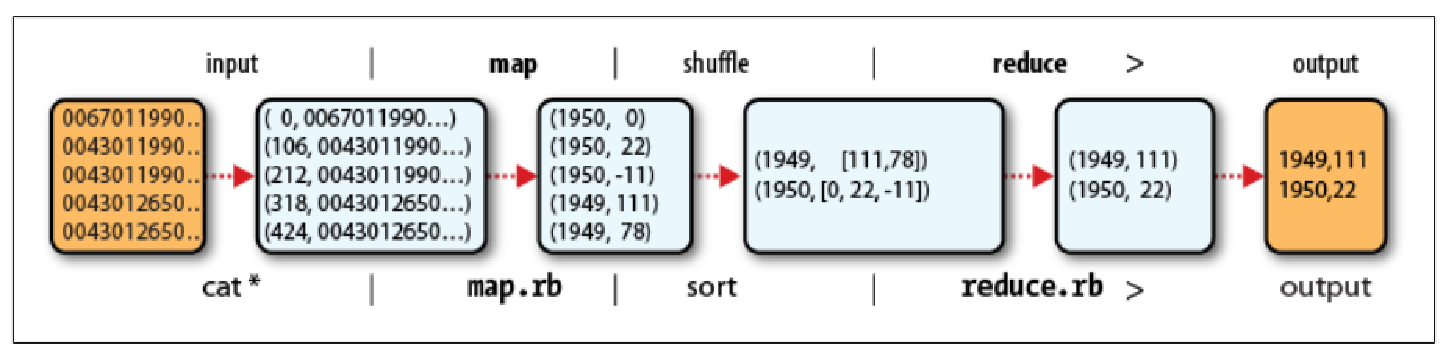
\includegraphics[width=\textwidth,height=\textheight,keepaspectratio]{./Figures/map-reduce.pdf}
    \rule{35em}{0.5pt}
  \caption{MapReduce logical data flow \cite{tom3}}
  \label{fig:map-reduce}
\end{figure}
%\end{verbatim}


\section{Hadoop}
% Lalith - The name Hadoop is not an acronym; it is made-up name by kid of Doug Cutting calling his yellow elephant toy “Hadoop”

Hadoop is an open source implementation of MapReduce programming model used to process huge datasets. Hadoop was created by Doug Cutting, the creator of Apache Lucene, the widely used text search library\cite{tom3}. Hadoop does the process of huge datasets in key/value pattern search. Where key is the data to be searched and value is the result of search for specific key. 

 Typically, datasets to be processed by Hadoop is large enough. Hadoop splits large data set into small fixed size chunks of data, called MapReduce jobs. To process the jobs, Hadoop splits jobs into smaller units called "Tasks", thus, a single job may consist one or many tasks. Using scheduler, tasks are scheduled for process and execution on the machines called datanodes. 
 
 Though Hadoop can run on single machine, but as it is used to process huge datasets, a set of machines forming Hadoop cluster is used to process data. The machines in Hadoop cluster works in master-worker pattern.The detail about machines in Hadoop cluster is explained in "Namenode and Datanode" section of this chapter. Hadoop Distributed File System (HDFS) is used by Hadoop to store and retrieve the data. HDFS has bigger size of data blocks then normal operating system file systems. The detail about HDFS‌ is explained in "HDFS" section of this chapter.   

There are two versions of MapReduce deployed in Hadoop, called MapReduce version 1(classic MapReduce) and MapReduce version 2( Yarn). The data process on each MapReduce version is processed using different components and techniques. The detail for each of these MapReduce versions are explained in \ref{MapReduce Versions}. Before explaining to detail of how does Hadoop works, here are some terms that helps the understanding of Hadoop/MapReduce data process: \\

\textbf{Job} MapReduce job is unit of work that needs to be processed by set of computers, in this case Hadoop cluster. It consist of input data ( raw data to be processed) , job configuration information and MapReduce program. 

\textbf{Task}‌ To run the jobs, Hadoop divides it into smaller units, called tasks. Tasks are real data that is processed in the system. There are two types of tasks: map tasks and reduce tasks.

Both, map and reduce tasks are predefined user functions, that is used to process data. For example, a map task reads the input data and searches for key in that data. The result of map tasks are redirected to reducer tasks/function, to sort and write the output values. 

\textbf{Job Size}  
 The default job size is 64 MB, which is equal to HDFS block size. Such job size is good for Rack Locality Feature of Hadoop. The job size is configurable and depends on job type and requirement may change to bigger or smaller size. If the job size is very small , then the job creation and map creation time will dominant the over all execution of job. having many small jobs mean that the execution time for each job is smaller comparing to large input. So if we run the small jobs in parallel on Hadoop cluster, the total time of processing all small jobs will be smaller than total time to process large input data set.\\ 


\subsection{HDFS}


 HDFS is the file system component of Hadoop which stores large data sets across cluster of computers in reliable and distributed manner. HDFS is designed to stream data in high bandwidth to user applications.
“HDFS is a filesystem designed for storing very large files with streaming data access patterns, running on clusters of commodity hardware” \cite{tom3}.According to \cite{tom3} HDFS‌ is designed to accommodate the follow:

\textbf{Very Large Files} 
  The “very large” in this context refers to files in size of hundreds of gigabytes or terabytes.

\textbf{Streaming Data}
  The efficient data processing idea behind HDFS design was based on write-once and read many times. Typically, dataset is generated or copied from source and process/query is executed on large proportion, if not all, of dataset. Therefore  the time to read the whole file is more important than reading the first record. 
  
%\subsection{Common \LaTeX{} Math Symbols}
\textbf{Commodity Computers}
   HDFS does not require expensive highly-available and reliable hardware. It is designed to run over cluster of commodity hardware (commonly available hardware from multiple vendors) where the  failure chances of hardware is very high. For case of hardware failure, HDFS is designed to continue process and work without noticing the user application from hardware failure.As the idea behind HDFS design is for large data files and the read time for the whole file is more important,thus HDFS will not work so well for low latency applications and small files. \\
 
 Not for each and every data and application HDFS‌ is fair data storage and retrieve method. Below are examples of cases where HDFS‌ may not work well for applications that fall into below categories. \  

\textbf{Low-latency data access}
Applications that requires low latency in tens of milliseconds, will not work well using HDFS.
The idea behind HDFS was for data with high throughput, loading large files, where total load time of a large file is critical.
 
\textbf{Lots of small data}
The information about data files stored and processed by Hadoop is stored as data called inode data. The inode data and list of blocks belonging to each file is called metadata. The namenode stores the filesystem metadata in random access memory (RAM). The number of files in namenode is limited by memory size. Each file, directory, and block takes 150 bytes in memory, so, it is feasible to have millions of files, but billions is beyond the capacity of available RAM.
   
\subsubsection{HDFS Blocks}
 
The minimum amount data or sequence of bytes (or bits) that disk can read or write is called disk block size. The size of disk block is usually 530 Bytes . To read and write data into blocks, filesystem blocks which are in size of kilo bytes are created on top of disk blocks. Generally, the disk blocks are transparent to filesystem.\cite{tom3} 
HDFS also has the concept of block; it is default block size is 64 megabyte. The size of HDFS block can be modified to larger number for example 128 megabytes or 512 megabytes. HDFS breaks the large file into fixed size chunks called HDFS blocks. Each block is stored independently in the cluster. For small file chunks, full capacity of HDFS is not occupied by HDFS. 

The time to read and write on disk depends on two factors called seek time and data transfer rate of the disk. The time needed to move HEAD (data reader or write component of disk) to the block from where it should read or write is called seek time. The amount of data that disk can read and transfer in second is called disk transfer rate which is usually calculated as megabytes per second. HDFS blocks are large compared to disk block size, this is to reduce the seek time of the disk. For large blocks, the data transfer time is significantly bigger compared to seek time to move to beginning of the block, thus time to transfer multiple files is equal to disk transfer rate.

It is not necessary that all blocks of the file to be placed on same single disk.  So, an advantage of the block structure is that if a file is larger than available capacity of single disk in the cluster, it can be stored across multiple disks in the cluster. 

%----------------------------------------------------------------------------------------


\subsection{Namenode and Datanode}

As explained in \cite{tom3}, HDFS cluster consist of two types of nodes which operates in master-worker pattern: a namenode (the master)and number of datanodes (workers). The total number of datanodes and namenode form a HDFS cluster. The namenode is responsible to store and manage filesystem namespace and the metadata for all files and directories in the tree. The information is stored in local disk in two different files "namespace image" and "edit log".

  Datanodes are workers that stores and retrieves data when they are told by namenode. The datanodes updates the namenode with list of data blocks that they are storing. All nodes in a Hadoop cluster communicate with each other using TCP-based protocols(TCP-based RPC‌ framework). To ensure reliability of data, multiple copy of data is stored on across multiple data nodes. By default three copy of the same data is stored.
   

All the information about filesystem is stored on namenode. The namenode knows all the datanodes on which the blocks for a given file is located. In case, if namenode data is erased ( due to failure or any other reason), then, all the files on file system is lost because there is no way of how to reconstruct data blocks. There for , having resilient namenode to failure and Hadoop provides two mechanism for this.
 

The first way is to configure Hadoop in a way that it write the steady state of the namenode to multiple filesystems as back up copy. The writes are atomic operations that can write to local disk and to a remote Network File System (NFS) mount.


As second solution, it is possible to run another namenode as secondary namenode to merge the image-space image with edit logs in order to prevent edit log files from becoming too large. Since secondary namenode requires as much CPU and memory as namenode (primary namenode) , usually, it runs on separate physical machine.The secondary namenode keeps copy of the merged namespace image , and this copy can be used in case of namenode failure. Usually, when namenode fails, copy of namenode data which are on NFS is copied to secondary namenode and runs secondary namenode as new primary.


   


%----- Data -----
%Hadoop stores meta-data and application data separately. The Meta data is stored in server machine so called Name Node. The user %application data is stored on other servers so called Data Node(s).  The advantage of this strategy is that data transfer is %multiplied and there are more chances to locate computation near the data (Data Locality)\cite{sailfish}.


\subsection{Schedulers}

Hadoop uses scheduling algorithm to assign jobs/tasks to nodes and executed them. The default Hadoop scheduler  used first in first out mechanism for submitted jobs. It means, the jobs were manager in queue structure,  and the first submitted jobs were scheduled for execution on the cluster. After completion of first job, the second job, and so on, jobs were executed. The scheduler is one of the key factors that can improve the performance of Hadoop, thus, literature suggested optimization to Hadoop scheduler. The performance and side effects of optimized Hadoop scheduler like Capacity Scheduler, Fairshare Scheduler and Speculative task execution is analysed in this thesis work. Detail explanation about Hadoop schedulers are covered in \ref{Hadoop Optimization} section. 



 



%----------------------------------------------------------------------------------------

%\section{Hadoop Schedulers}

\section{MapReduce Versions}

To coordinate and manage the process and execution of jobs, few more components are used by Hadoop. The component used in Hadoop depends on Hadoop versions. Up to now, Hadoop takes advantage of two versions of MapReduce, called MapReduce version 1, and MapReduce version 2(YARN). Both versions have different components and methodology to process the jobs. 

\subsubsection{MapReduce Version 1} 
MapReduce Version 1, which is also called classic MapReduce has the following methodology to run jobs (brief):

  - Client is the one that submits jobs to MapReduce to be processed. 
  - The JobTracker is the component used to coordinate the jobs for process. 
  - The TaskTracker is the component to run the tasks (as explained in \ref{Hadoop}
     tasks are small splits of jobs).
  - A scheduler is used to schedule the tasks for process.
  - HDFS‌ is used to store and retrieve the data.  
 
The figure \ref{mrv1}  explains the structure of MapReduce version 1. 

\begin{figure}[htbp]
  \centering
    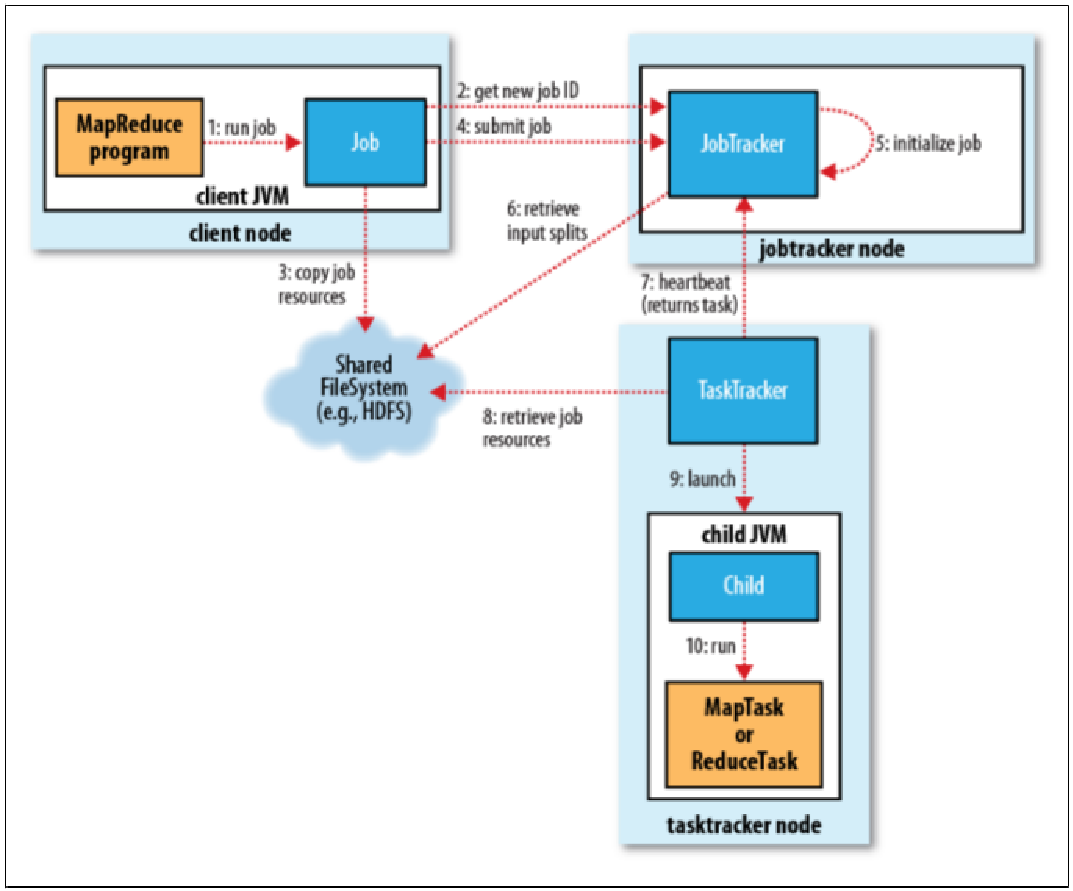
\includegraphics[width=10 cm,height=10 cm]{./Figures/mrv1.pdf}
    \rule{30em}{0.5pt}
  \caption{MapReduce Version 1 Architecture \cite{tom3}}
  \label{mrv1}
\end{figure}
 


Detail:
Usually the data to be process by Hadoop is very large dataset. Hadoop divides this large dataset input to small fixed-size "input split” or “split”. Each split is called MapReduce job. The splits are fed as input to user defined map function. Map functions read each record of input split and process it.\\

Job execution are controlled by two components of Hadoop called JobTracker and TaskTracker. JobTracker is responsible to run all jobs on system. It coordinates job execution by scheduling tasks on tasktracker. The JobTracker maintains record about status of each job and monitors the progress of each task. The TaskTracker executes tasks on nodes and sends progress report to JobTracker. In case if task execution failed, the JobTracker is the one which reschedules the task on same or different TaskTracker.\\




















\subsubsection{MapReduce version 2 (Yarn)}

For clusters with more than 4,000 nodes, MapReduce version 1, had scalability bottlenecks. To over come this issue , the new version of MapReduce called Yet Another Resource Negotiator (YARN) was created by Yahoo!‌ at 2010 \cite{tom3}.\\  

To overcome the shortcoming of MapReduce version 1, YARN splits the functions of JobTracker into two separate components. As explained in \ref{MapReduce version 1}‌, JobTracker is responsible for job scheduling and task progress monitoring, YARN‌ uses application manager and resource manager as two seperate daemons for these functions. \\

\begin{figure}[htbp]
  \centering
    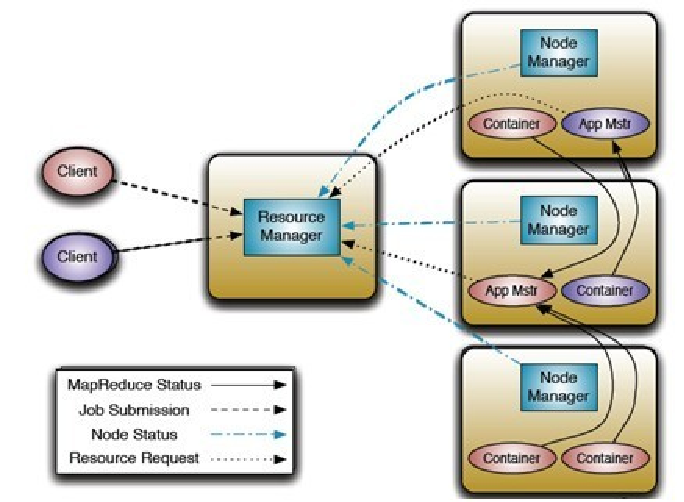
\includegraphics[width=10 cm,height=10 cm]{./Figures/yarn.pdf}
    \rule{25em}{0.5pt}
  \caption{YARN‌ architecture \cite{yarn}}
  \label{yarn}
\end{figure}

As illustrated in figure \ref{yarn}, there is single Resource Manager and per-application Applications Master. Application could be single job or group of jobs. The per-application master, negotiates for resources with resource manager and works with node manager to monitor tasks. There is an agent per datanode (worker machine) called node manager, that  monitors the resource usage for application running on datanode, and submits the status report of each node to resource manager.\\
 
Resource manager is responsible to manage resource usage across cluster. It has two main components:
The Scheduler, which is responsible to allocate resources to applications and does not perform the monitoring or tracking status of the application. The scheduler performs provides the resources based on resource requirements of applications. The abstract notion \i{Container} is used for resource, where resource could be incorporate of elements like memory, cpu, disk, network etc. The scheduler has plugin policy, based on resource can be be configured and shared among different applications for example capacity and fairshare schedulers. The performance evaluation and side effects of schedulers are the core of study in this thesis.\\

The ApplicationManager is the entity that accepts the submitted jobs, negotiates for the container to execute per-application ApplicationMaster and in case of failure, restarts the ApplicationMaster. The ApplicationMaster is responsible to negotiate required resource container for application(job or jobs) from scheduler, track and monitor the progress of the application. The ApplicationMaster is created per application and runs for the duration of its application, and finishes after complete process of application.  


YARN‌ is compatible with MapReduce version 1, all jobs of MapReduce version just needs re compilation to be executed on YARN \cite{yarn}.   



  




\section{Cloud Computing}

Cloud Computing is a distributed computing paradigm that enables the provision of available, scalable and reliable on-demand resources over a network, primarily the Internet \cite{nist}. Applications, networks, platforms , storage, processing power , service , etc can be resources in cloud computing. Resources can be provisioned and released with minimal management interaction of the provider. The composition of resources , mostly as virtualized pool of resources are provisioned to customer and can be released with minimal management interaction of provider or customer. Since, customers are unaware of how and where are the resources, the term "cloud" is an abstraction paradigm used for such services. 

\subsection{Service Models}
The classification of cloud computing paradigm according to the level of abstraction and control provided to them, offers several types of services. A well known classification of cloud services , adopted by United States National Institute of Standards and Technology (NIST)‌, is explained below: 


\textbf{Software as a Service (SaaS)} SaaS model provides the facility to consumer to use software applications running in cloud infrastructure. To access the services, a user interface through which user can access the services from any device using applications such as web browser(e.g.,web-based email). The infrastructure on which service is running, is owned and managed either by provider or third party and consumer has limited or no control over underlying resources. Examples of SaaS providers are: Google Docs, Dropbox and GitHub. \\  


\textbf{Platform as a Service (PaaS)} PaaS model allows the consumers to create,use and deploy 
applications on the cloud provider's infrastructure. Consumer can use programming languages and tools supported by provider to create and deploy applications. The control level given to client is
 more than SaaS, but limited to control over deployed applications and to configuration 
settings of application hosting environment. Examples of PaaS providers are: Google App Engine, Microsoft Azure.\\    



\textbf{Infrastructure as a Service (IaaS)} IaaS provides the capability to the consumer to use fundamental comuting resources such as processing, storage, networks. The consumer is also able to deploy arbitrary software including operating system on the cloud. The consumer has control over software, operating systems and deployed applications, but the physical infrastructure that runs the services is owned by provider. Typically, the physical resources are shared among multiple users or organizations by virtualization hypervisor. Examples of IaaS‌ providers are: RackSpace and Amazon Elastic Compute Cloud (Amazon EC2). \\ 


\subsection{Deployment Models}

The classification of cloud computing can be done based on deployment models. NIST \cite{nist} defined the following four categories as deployment model for cloud computing:

\textbf{Public Cloud} The cloud is made available to general public or groups of people and industries. The infrastructure is either owned by cloud provider or third party. 
  
\textbf{Private Cloud} The cloud is operated exclusively by single organization. The cloud maybe managed and owned by other organization or third party. 
 
\textbf{Community Cloud} The Cloud is shared by several organizations that have common interests such as share mission , security or university campus. It maybe owned and managed by organization forming community or a third party. 


\textbf{Hybrid Cloud} The composition of two or more clouds deployments by standardized technology to single cloud infrastructure , that provides portability is called hybrid cloud. \

















 
% Chapter Template

\chapter{Hadoop Optimizations} % Main chapter title

\label{Chapter3} % Change X to a consecutive number; for referencing this chapter elsewhere, use \ref{ChapterX}

\lhead{Chapter 3. \emph{Hadoop Optimizations}} % Change X to a consecutive number; this is for the header on each page - perhaps a shortened title

%----------------------------------------------------------------------------------------
%	SECTION 1
%----------------------------------------------------------------------------------------
  To improve the performance of Hadoop, literature suggested various optimizations. This chapter explains the suggested and deployed optimizations of Hadoop schedulers. 
  
  Hadoop is a MapReduce application that processes large datasets (that are divided to small fixed sizes units called jobs)on cluster of commodity computers in parallel and distributed fashion. Hadoop scheduler is the component that decides when and on which node to process the jobs, so the performance of Hadoop is closely tied to its scheduler. The optimizations like Capacity Scheduler, Fairshare Scheduler, Speculative Task Execution and Longest Approximate Time to End(LATE) are explained in this chapter. 
   
 
 
 \section{Capacity Scheduler}
 
Though organizations can have their own private compute resources with sufficient capacity to execute jobs on, but such private resources may be expensive and lead to low utilization of resources. Capacity Scheduler is pluggable MapReduce scheduler that is designed to allow multiple tenants to share large Hadoop cluster securely and to maximize utilization of the cluster. It is cost effective for the organization to share clusters and run jobs comparing to having their own private clusters.\\ 

 Using capacity scheduler, the organizations fund the Hadoop cluster collectively, and obtains their share. The available resource in the Hadoop cluster is partitioned and  guaranteed  minimum share for each organization is provided. In addition, organization can access more then limited share only when the cluster resource is not used by other organization. This mechanism provides elasticity for organizations and maximizes the cluster utilization. It means, if other organizations does not use the cluster, then any organization can use entire (not limited to its own share) cluster resources for its computational jobs as long as they are the only one organization submitting jobs to the cluster.\\
 
 As the cluster is shared among organization, this leads to strong cooperation for multi-tenancy to guarantee minimum share limit of each organization. To avoid more than limit consume of resources  by single job or user that affects other organization's share, capacity scheduler provides safe-guards that limits the user or job access to its share.\\
 
  The capacity scheduler , manages users and jobs in queue structures. Typically the queues are setup by administrator, where multiple queues are created for job management. Each organization may own one or more queues where they can submit the jobs. Each queue is provided limited portion of computational resources to process the jobs. The amount of computational resources depends on economical share of the cluster for an organization. The more economical share you have , the more computational resources are available for your job process.  Typically, the resources are divided on percentile base for each queue and if there is single organization submitting the jobs, it can use entire computational resources of cluster. 
 
 % To be added in Apendix:‌ As mentioned in above paragraph, capacity scheduler is pluggable Hadoop MapReduce job scheduler which is available as JAR file in the Hadoop tarball under contrib/ capacity-scheduler directory. It is  possible to build scheduler from source by executing ant package, and source package is available under build/contrib/capacity-scheduler.\
 
 Capacity schedulers supports the following features:
 

 

 \textbf{Capacity Guarantee} Capacity scheduler supports multiple queues, the organizations submit jobs to their relevant queue(s). The cluster resources is allocated between all the queues based on their economical share of the cluster. It means, certain amount of resources are dedicated to each queue, where job from that queue can use these resources. There could be soft or hard limit between resources of the queues, configured by administrator. Where soft limit means that queue can access more then limited capacity if the others does not use the resource. Hard limit refers to situation where organization can use only their own share of the resources, and not more. 


 
 \textbf{Security} In order to prevent unauthorized user to submit jobs to queue, strict access control lists are applied to each queue. The safe-guards can be used to ensure that users can not view or modify jobs from other users.   
 

\textbf{Elasticity } Free resources can be allocated to queues that are in demand of resources. For any queue, that has a share of computational resources, and does not need it any more or for period of time, its share is allocated to other queues that are in demand for resources. The scheduler allocates the resources to queues that are running lower than their share and are in demand for further computational resources. This mechanism maximizes the utilization of resources and ensures that resource are available in elastic manner. 


\textbf{Multi-tenancy } To ensure that cluster resource is not monopolized by single job, user or queue, limits are provided which ensures that the system ( in Hadoop version 1 JobTracker ) is not overwhelmed by too many tasks or jobs. 

\textbf{Operability } Users and administrators can view current allocation of the queues of the system through console. It is also possible to change queue modification during run time without disruption to users. 


\textbf{Resource-based Scheduling } Resource intensive jobs are those that require or can demand for higher-requirement than default. Capacity Scheduler can accommodate applications or in particular jobs with different resource requirement. Memory is the only resource currently supported by Capacity Scheduler. 

\textbf{Job Priorities } Though a running job can not be preempted by any other job, but it is possible to assign higher priority to a job within the queue. Jobs that have higher priority will have access to queue's share of resources faster than jobs with lower priority. By default, priority is disabled in capacity scheduler. 


\section{Fairshare Scheduler}

Fairshare scheduler is pluggable MapReduce Hadoop scheduler that maintains separate queues for user groups (pools). Resources are allocated to jobs, in a way that on average every job gets fair share of resources over time. If there is single job running, then, it can utilize full resources of the cluster. For new submitted jobs, the slots that become free will be allocated, this mechanism provides opportunity that each job consume on average roughly the same amount of resources. Unlike default Hadoop scheduler that maintain queue of jobs, fairshare scheduler lets short jobs to complete in reasonable time and also it does not starve long jobs.  \cite{dynamic} \cite{fair}\\

 
The fairshare scheduler maintains jobs into pools, initial fair distribution of resources across multiple pools are assigned to these pools in order to limit their access to resources. In addition to provision of fair share of resources, fair share scheduler can provide minimum guaranteed amount of resources ( or computer time of CPU) to each pool to ensure that each user, pool gets sufficient amount of resources. If a pool completed its jobs and does not need the resources,excess resources is evenly distributed among other pools.\cite{fair}\\

 By default there is one queue per user so that all users can get equally same fraction of total resources.The setup of job pool is possible based on Unix user groups or any other jobconf property.Within each queue, jobs can be scheduled as FIFO or fair share schedule. Fairshare scheduler can support job priority, where priority is weight that identifies fraction of total compute time for each job. In addition,  inter-queue job priority is also supported by fair-share scheduler.\cite{fair}
 
 
 \textbf{Task Preemption } In the case minimum share of a pool is not provided, after waiting for certain period of time, the scheduler may kill a task from other pool(s) to provide minimum share to pool.Killing task of other jobs is called task preemption.It is also possible that preemption happen if a pool is below its half share for configurable time-out period.Usually time-out value is higher than minimum share time-out preemption.\cite{fair} 
 
In both cases of above preemption , the fair share scheduler kills most-recently-launched tasks from over-allocated jobs, to minimize wasted computation. Since Hadoop jobs are tolerated to losing tasks, killing tasks does not cause jobs to fail but causes them to take longer to finish.\cite{fair}
 














\section{Speculative Execution}

The goal of speculative execution is to reduce the job completion time by speculating the tasks from straggler machines. The tasks are categorized into below 3 categories. If there is free slot on a node, then a task is selected according to the category number from one of these categories.  

\textbf{Failed Tasks }  If a task fails multiple time , due to a bug and stop the job, such task is marked as "failed task" and given highest priority. 

\textbf{Non-Running Tasks } These are fresh tasks that has not being executed on any node yet. For maps, data-locality is considered and tasks that are closer to the node is performed first. 

\textbf{Speculative Tasks } To find speculative task,the progress of task is monitored by Hadoop with a progress score between 0 and 1.Map progress depends on input data read and its progress score is fraction of input read data. The reduce phase compromise three sub phases where each sub-phase is counted as 1/3 of progress report. The three sub-phases of reduce phase is explained bellow: \\

\begin{itemize}
\item{Fetching of map outputs, also called copy phase.}
\item{Sorting of map outputs by key, also called sort phase.}
\item{Applying user-defined function to the list of map outputs with each key, also called reduce phase. }
\end{itemize}
	

In each sub-phase of reduce, the score is fraction of data processed. For example, a task halfway through the copy phase has a progress score of 1/2 * 1/3 = 1/6 , while a task halfway through the reduce phase scores 1/3 + 1/3 +(1/2 * 1/3)= 5/6.

\textbf{Straggler}  For map tasks and reduce tasks average of their progress score is defined as threshold by Hadoop.If progress score for a task is less then the the threshold of its category (maps or reduces) minus 0.2, and it has run for at least 2 minutes , it is marked as straggler. All the tasks below the threshold are considered as slow and the scheduler runs at least one speculative copy of these tasks at time\cite{mat1}. 
 




%%%%%%%%%%%%%%%%%%%%%%%%%%%%%%%%%%%%%%%%%%%%%%%%%%%%%%%%%%%%%%%%%%%%%%%%%%%%%%%%%%
%%%%%%%%%%%%%%%%%%%%%%%%%%%%%%%%%%%%%%%%%%%%%%%%%%%%%%%%%%%%%%%%%%%%%%%%%%%%%%%%%%

\section{LATE Scheduler}

LATE‌ is the abbreviation for scheduling algorithm of Hadoop called Longest Approximate Time to End (LATE), which is robust to environment heterogeneity and can improve the response time of Hadoop cluster by factor of 2\cite{mat1}. \\

The idea behind LATE‌ is to speculatively execute tasks, that are estimated to be completed in furthest  time in the future. It means, the finish time for tasks are estimated and those tasks that are going to finish in longest period of time in future, are speculatively executed. Not like normal speculative execution of tasks, where speculated tasks can be run on any machine, LATE‌ runs speculative tasks on faster nodes to complete speculative copy of task faster than original task. \\

To estimate the time left for task completion, the following heuristic is used by LATE:\\
 The tasks progress is monitored by scheduler, and marked with a \i{ProgressScore}, which represents the fraction of work processed from all the work. Where map task is calculated as single task, for reduce task,  the ProgressScore is the sum of \i{copy phase, sort phase, reduce phase}‌ where each phase represents 1/3 of total task progress.
  
 The \i{ProgressRate}‌is another factor estimated for each task, which is equal to \i{ProgressScore/ T}, T is the task duration time. The task completion time is estimated based on ProgressRate of each task, which is \i{ (1 - ProgressScore/ProgressRate) }. Maybe tasks has different ProgressRate, but the assumption in LATE‌ is the tasks has same ProgressRate.\\  
  
To run speculative tasks on fast nodes, an estimation against SlowNodeThreshold is calculated for every node, any node that are below SlowNodeThreshold is considered as slow node. Speculative tasks are only executed on fast nodes (not slow nodes) . SlowNodeThreshold is the percentile of speed comparing to total speed of nodes in cluster. Choosing percentile for SlowNodeThreshold is optional, but as per \cite{mat1}, their observation show better performance for setting SlowNodeThreshold to 25 percent.\\   

 To decide how many tasks to speculate simultaneously, a threshold called SpeculativeCap is defined. The SpeculativeCap is the total number of slots where tasks can be speculatively executed. If there is less than SpeculativeCap tasks are speculative tasks are running, and there is free node to run tasks, for task assignment the following decision is made:\\
 \begin{itemize}
 \item{If node is slow(total progress is lower than SlowNodeThreshold) then ignore the request of node for task execution.}
 \item{Estimate the time left for running tasks that are not speculated and rank them for speculative execution.}
 \item{Run the copy of task with highest rank (lowest progress rate comparing to SlowTaskThreshold). }
  
 \end{itemize}

 
 The decision to choose proper values for parameters of LATE‌ has important role on overall job completion time. As per \cite{mat1}, they obtain best performance of LATE by setting SpeculativeCap to 10\% of available task slots, SlowNodeThreshold to 25\% percentile of node progress. 
 

 
\subsection{Advantages of LATE}

The native Hadoop scheduler mechanism is to consider any task that is below the fixed threshold as slow task and treat them equally for speculative execution. While, LATE relaunches the slowest task and small number(at maximum as SpeculativeCap) of tasks to limit contention for shared resources.LATE mechanism is to prioritize among slow tasks on how much they hurt job response time and rank them for speculation priority.\\
Hadoop native scheduler assumes that nodes are homogeneous and any candidate node for task execution is likely to be a fast node. In contrast, LATE takes into account node heterogeneity by ranking some nodes as slow node(nodes below SlowNodeThreshold are marked as slow node)and assigns new tasks only to fast nodes.\\
Hadoop native scheduler focuses on progress rate and speculatively executes any slow task. LATE focuses on estimated time left and speculatively executes only tasks that will improve job response time. For example,if task A is 5x slower than the mean but has 90 percent progress, and task B is 2x slower than the mean but is only at 10 percent progress, then task B will be chosen for speculation first, even though it is has a higher progress rate, because it hurts the response time more. Therefore , LATE provides opportunity for slow nodes to be utilized as long as this does not hurt job response time which is unlike of progress rate base scheduler that always re-executes task from slow nodes.      

































% Chapter Template

\chapter{Methodology } % Main chapter title

\label{Chapter4} % Change X to a consecutive number; for referencing this chapter elsewhere, use \ref{ChapterX}

\lhead{Chapter 4. \emph{Methodology}} % Change X to a consecutive number; this is for the header on each page - perhaps a shortened title

%----------------------------------------------------------------------------------------
%	SECTION 1
%----------------------------------------------------------------------------------------

\section{Objective of The Work}

The focus of this work is on performance evaluation of Hadoop schedulers and side effects of collocated nodes. The goal of the work is to analyse the performance of the optimizations added to Hadoop schedulers such as capacity scheduler, fairshare scheduler including speculative task execution. Targeted set of scheduler is used as case study, and experiment and evaluations are done for specific schedulers. The study provides performance evaluation for capacity share scheduler and fairshare scheduler evaluation. In the context of this work, the performance of scheduler refers to job completion time in Hadoop cluster. The lower the job completion time is the better performance is evaluated and vice versa. Aside from job completion time as measure for schedulers performance, the fairness of job completion time is also evaluated. The analysis include findings about schedulers behaviour that causes performance degradation for job completion.\\
 
 The run of virtualized Hadoop cluster, where every VM‌ is running on one physical machine, is evaluated as baseline case. Not all the time stand alone Hadoop cluster is running on physical machines, so beside the scheduler performance in baseline, performance is analysed when two datanodes are collocated from the same cluster and when two datanodes are collocated from different clusters. The purpose of the collocated datanodes is to analyse how the placement of Hadoop nodes can affect the performance of the Hadoop. 


\section{Methodology}

The goal of the work is to analyse Hadoop schedulers performance and side effects of collocated Hadoop datanodes. To achieve the goal, a placement strategy and set of schedulers  are defined for the experiments. In this thesis, an experiment consist of set of schedulers, along with node placement strategy with workload execution on experimental environment. \\

The optimized schedulers that are selected for all the experiment are capacity share and fair-share schedulers. These schedulers are selected because they both provide the opportunity for multi-tenancy of resources among organizations. In addition to default behaviour of scheduler which performs speculative task execution, the non speculative behaviour of the schedulers are also evaluated. Overall, the scheduler set includes two schedulers in two different status which forms four cases in total:\\
 \begin{itemize}
 \item{Capacity share scheduler with speculative task execution which is referred as "cpt" in plots.}
 \item{Capacity share scheduler without speculative task execution which is referred as "cpf" in plots.}
 \item{Fair-share scheduler with speculative task execution which is referred as "fst" in plots.}
 \item{Fair-share scheduler without speculative task execution which is referred as "fsf" in plots.}
 \end{itemize}
	
The placement strategy is about where to locate the datanodes and consist of three different cases of baseline,collocated datanodes, collocated clusters.\\

\textbf{Baseline } In this case, Hadoop nodes are placed as one node per physical machine. Not any machine is shared between two datanodes. The experiment is evaluated for the complete set of Hadoop schedulers used as baseline. The result of the experiment from baseline case is used as base performance of schedulers and two more cases are compared to baseline to find the effect of collocation of datanodes.  In total there is single Hadoop cluster running on bare-bone hardware using VMs.\\ 
 
\textbf{Collocated Datanodes} This is the case where more than one datanodes are placed on one physical machine. In total two datanodes are placed on single physical machine. Both datanodes located on one physical belongs to same Hadoop cluster. The goal is to find out how collocation of data nodes from same Hadoop cluster can affect the performance of Hadoop scheduler?, In total there is single Hadoop cluster running with two datanodes on every machine using VMs. \\
 
\textbf{Collocated Hadoop Clusters } The collocated Hadoop cluster is similar to Collocated datanodes case with difference that it has two Hadoop clusters launched on computational resources. In this case a total of two datanodes share a single physical where each datanode belongs to a separate Hadoop cluster. The goal of this placement is to analyse the performance impact of datanode from one cluster on the datanode from another cluster. In total two there are two Hadoop clusters running  with two datanodes of different cluster on every physical machine using VMs.\\  

\textbf{Fairness } Fairness represents the time difference between job all job completion time. The fairness is calculated as maximum job completion time minus minimum job completion time for each run during experiment. \\

The total number of VMs used in baseline and collocated datanodes are equal. While in baseline every datanode VM is spawned on one physical machine and in collocated datanodes two datanode VMs are placed on one physical machine. The total number of physical machines in collocated datanodes case, used for datanodes placement  is half of the number of physical machines used for datanodes in baseline case. The collocated cluster case is similar to run of two baseline at the same time. It means, each Hadoop cluster in collocated cluster case is exactly the same as single baseline Hadoop cluster.  
  


\section{Work Scope}

The scope of the thesis is limited to few cases of Hadoop optimizations, and node placement effects. The results of the thesis is limited to experimental environment,used workloads, tools, softwares, and physical machines. The results from this thesis does not guarantee that Hadoop optimization will have same results in every other scenario or environment. Some limitation of the work is explained in next paragraphs. \\

 This thesis addresses the performance evaluation and side effects of Hadoop optimizations. The optimization refers to optimized Hadoop schedulers like capacity scheduler, fairshare scheduler, and speculative task execution. The schedulers can be configured in different ways like queue configuration, assigning percentile of resources and so on, but this thesis work is limited to default queue configuration of the schedulers. The only change of parameter is the number of reducers changed for experiments. I select YARN‌ as optimized Hadoop version, and tested all the schedulers  using YARN. \\

The side effects here stands for effect of multiple nodes sharing the same physical machine. I placed two datanodes running on two VMs on top single physical machine to see how the datanodes placement have side effects on Hadoop performance. The placement of two datanodes from same cluster and from different clusters were tested to see the difference of side effects for each case.It is possible to configure namenode in a way, to act as both namenode and datanode. In the experiments , the namenode was only acting as namenode (not as datanode). The performance of scheduler is evaluated for the cases where all the datanodes are processing the data. The results of evaluation and side effects of Hadoop optimization is also limited by submitted jobs size and types.\\

There is single workload "terasort" used as workload and terasort benchmark is used for the performance evaluation of the schedulers. So, the results of the thesis is limited to "terasort" workload and this result may vary for Hadoop schedulers performance using other benchmarks. The thesis result is limited to results for used Ubuntu VMs on specified set of physical machine.  All the experiments were executed using Ubuntu VM and it was not ran on bare-bone hardware. it is possible that running the same experiments on bare-bone hardware provide different results.\\



\section{Experimental Environment}

The experiments are executed on test-bed environment. The environment consist of resources: physical machines, Ubuntu operating system, Hadoop application, OpenStack and tools/scripts to process and analyse the log data.\\


Each experiment consist spawning and installation of Ubuntu 12.10 Virtual machine on top of physical machines. For all the experiments, Hadoop-snap-shot-3 is configured and used as instance of Hadoop application to form Hadoop cluster.  After completion of Hadoop setup, using terasort, workload is generated and stored on datanodes. Once, the workload generation is completed, the terasort starts process to sort the data using Hadoop's scheduler. The performance of each and every scheduler for every placement strategy is analysed for the time duration that terasort sorts the generated workload. A set of metrics like job start time, end time, number of mappers and reducers, number of killed tasks, etc are collected for further analysis.\\    

For management of VMs, including installation and deletion, OpenStack software is used as tool. To automate the process of installation, configuration of VMs and nodes, and running terasort on Hadoop cluster, python scripts are used. The bash scripts collects the required metrics from the logs generated from Hadoop's performance. For further process and analysis of collected metrics, R was use as tool to analyse and plot the log data. The scripts are appended at the end of thesis to appendix.  


%-----------------------------------
%	SUBSECTION 1
%-----------------------------------
\subsection{Physical Resources}
A total number of seven(7) computer machines connected through central switch is used to run the experiments. All the computers are connected using Gigabit Ethernet port to the switch. Each computer has sixteen(16)GB of RAM(Random Access Memory). The computers are equipped with eight(8) CPUs(Central Processing Unit), where the speed of each CPU is approximately 2,3 GHZ.The system uses 10 GB of disk space to store the virtual machine and Hadoop software. Additional mounted hard disk space of seventy two(72) GB is provided as NFS(Network File System) storage to each computer. 

%-----------------------------------
%	SUBSECTION 2
%-----------------------------------

\subsection{Terasort}
Terasort is a benchmark tool used to sort large set of generated data. It is a standard tool to generate and sort large data sets using random data. The tool was used by Yahoo!‌ at 2009 to sort one terabyte of data on 9000 machines using Hadoop. The two core component of terasort is Teragen and Terasort. 

\textbf{Teragen} - Generates the random data that is used as input data for terasort.The data is generated in rows and the format of 
row is "<10 bytes key><10 bytes row-id><78 bytes filler>". 
The keys are random characters from the set ‘ ‘ .. ‘~’, row-id is justified row id as a int and the filler consists of 7 runs of 10 characters from "A" to "Z". Teragen divides the number of rows by the desired number of tasks and assigns set of rows to each map.\ref{TeraByte Sort on Apache Hadoop Owen O’MalleyYahoo!}


\textbf{TeraSort} - It is implemented as a MapReduce sort job with a custom partitioner that uses a sorted list of n-1 sampled keys that define the key range for each reduce.


%----------------------------------------------------------------------------------------
%	SECTION 2
%----------------------------------------------------------------------------------------





\subsection{OpenStack}

OpenStack is developed by developers of cloud computing, it is open standard cloud operating system for public and private cloud operators. OpenStack consists of three core components:OpenStack Compute (code-name Nova), OpenStack Object Storage (code-name Swift), and OpenStack Image Service (code-name Glance).


\textbf{OpenStack compute} The OpenStack compute is designed to provision and manage large cluster of virtual machines. The software provides control panel for running instances, managing network and control of access via users.
 
\textbf{OpenStack Object Storage} The OpenStack Object Storage is used for creating petabytes of accessible data. It is a system for long term storage of large amount of static data. The data can be leveraged,updated or retrieved.For better scalability and redundancy, the data is stored in distributed manner with no central point of failure.

\textbf{OpenStack Imaging Service} Using image services, the clients can register new disk images.The image discovery is designed to facilitate the discovery,registration and delivery services of virtual disk to the users.               
              
 
The software called "OpenStack" is used as tool to create,store and manage virtual machines. We use it for our experiments. Initially, we spawned only Ubuntu VMs and configured it for Hadoop cluster to run terasort workload. After making sure, that VMs are running properly and sorts the workload, we create an image from  running VM to use it for further experiments. Basically, images are similar to clone of Ubuntu system that is capable to reboot, install, and configure for Hadoop clusters. Though, there were only Ubuntu virtual machine used for experiments but, within Ubuntu two different virtual machines images were configured which was called "Hadoop namenode image" and "Hadoop datanode image". Respectively, the images were spawned, configured and used to act as namenode and datanodes for experiments.\\ 

\subsection{Ubuntu Virtual Machine}

 
% Chapter Template

\chapter{Evaluation} % Main chapter title

\label{Chapter5} % Change X to a consecutive number; for referencing this chapter elsewhere, use \ref{ChapterX}

\lhead{Chapter 5. \emph{Evaluation}} % Change X to a consecutive number; this is for the header on each page - perhaps a shortened title

%----------------------------------------------------------------------------------------
%	SECTION 1
%----------------------------------------------------------------------------------------
This chapter is about the detail of the experiments, results, analysis and discussion of results. For better understanding of the experiments a structure is created where the experiment detail, objectives,results,fairness and discussion about every experiment is explained.  The experiments are performed for three cases of baseline, collocated datanodes and collocated clusters. For every placement cases of baseline and collocated datanodes single Hadoop cluster is used to sort the generated data. The collocated cluster case was experimented using two set of six VMs ( a set of six VMs per Hadoop cluster) for all schedulers. All the experiments, consists three placement cases of baseline, collocated datanodes and collocated clusters and for each placement, all of four schedulers cases "cpt","cpf","fst" and "fsf" performance is evaluated. In total, every experiment consists twelve (12) cases for all the placement and schedulers cases. Below settings were the same for all the experiments:

\begin{itemize}
\item{ Every experiment was executed five times.}
\item{ Every VM had the same amount of Hard drive, memory and CPUs.}
\item{ For each Hadoop cluster, the workload was 25 GB of data.}
\item{ Five jobs were submitted for each Hadoop cluster, each job size is 5 GB.}
\item{ Three copy of workloads were stored on datanodes.}
\item{ Total of six VMs, one as namenode and five other acting as datanodes formed a Hadoop cluster.}

\end{itemize} 

\section{Experiment 1}

 In experiment one, we sort the generated workload using terasort, without tuning any parameter of MapReduce.  In each Hadoop cluster, a total of five (5) jobs were submitted by single user, where each job size was five (5) GB of data, in total twenty five (25) GB of data. The data were replicated three (3) times across datanodes for reliability.Single user submitted five jobs to default root queue of Hadoop scheduler.  There were no special configuration of Hadoop scheduler.\\  
 
 


\subsection{Objectives}
  
  One of the objectives of the experiment was to find out what is the default performance result for terasort workload. It means, the number of mappers and reducers are not pre-specified, and Hadoop scheduler is allowed to use arbitrary number of mappers and reducers. The experiment was designed to analyse the default behaviour of Hadoop scheduler for terasort. It is also important to see by default, which scheduler has better performance and which scheduler has better fairness in comparison to other schedulers. We also wanted to analyse how is the affect of speculative task execution (which is one of the optimizations to Hadoop scheduler)‌ on the performance of Hadoop. The experiment also addresses the impact of collocation for default terasort workload.\\
 
  As this is the first experiment set, where we did not changed any parameter, so the result of this experiment is used to see how the parameter change on the other experiments affects performance of Hadoop.\\  

 
\subsection{Results}
 
  During the experiment, we find out that by default, terasort runs with single reducer. For experiment the total number of mappers were more than forty (40+) and single reducer. It means, to complete a task , output of all mappers should wait for single reducer to become free and process the data which causes delay in overall job completion time. The figure \ref{fig:exp_1_mean} illustrates the mean values for job completion time for each scheduler and placement cases.\\
 

\begin{figure}[htbp]
  \centering
    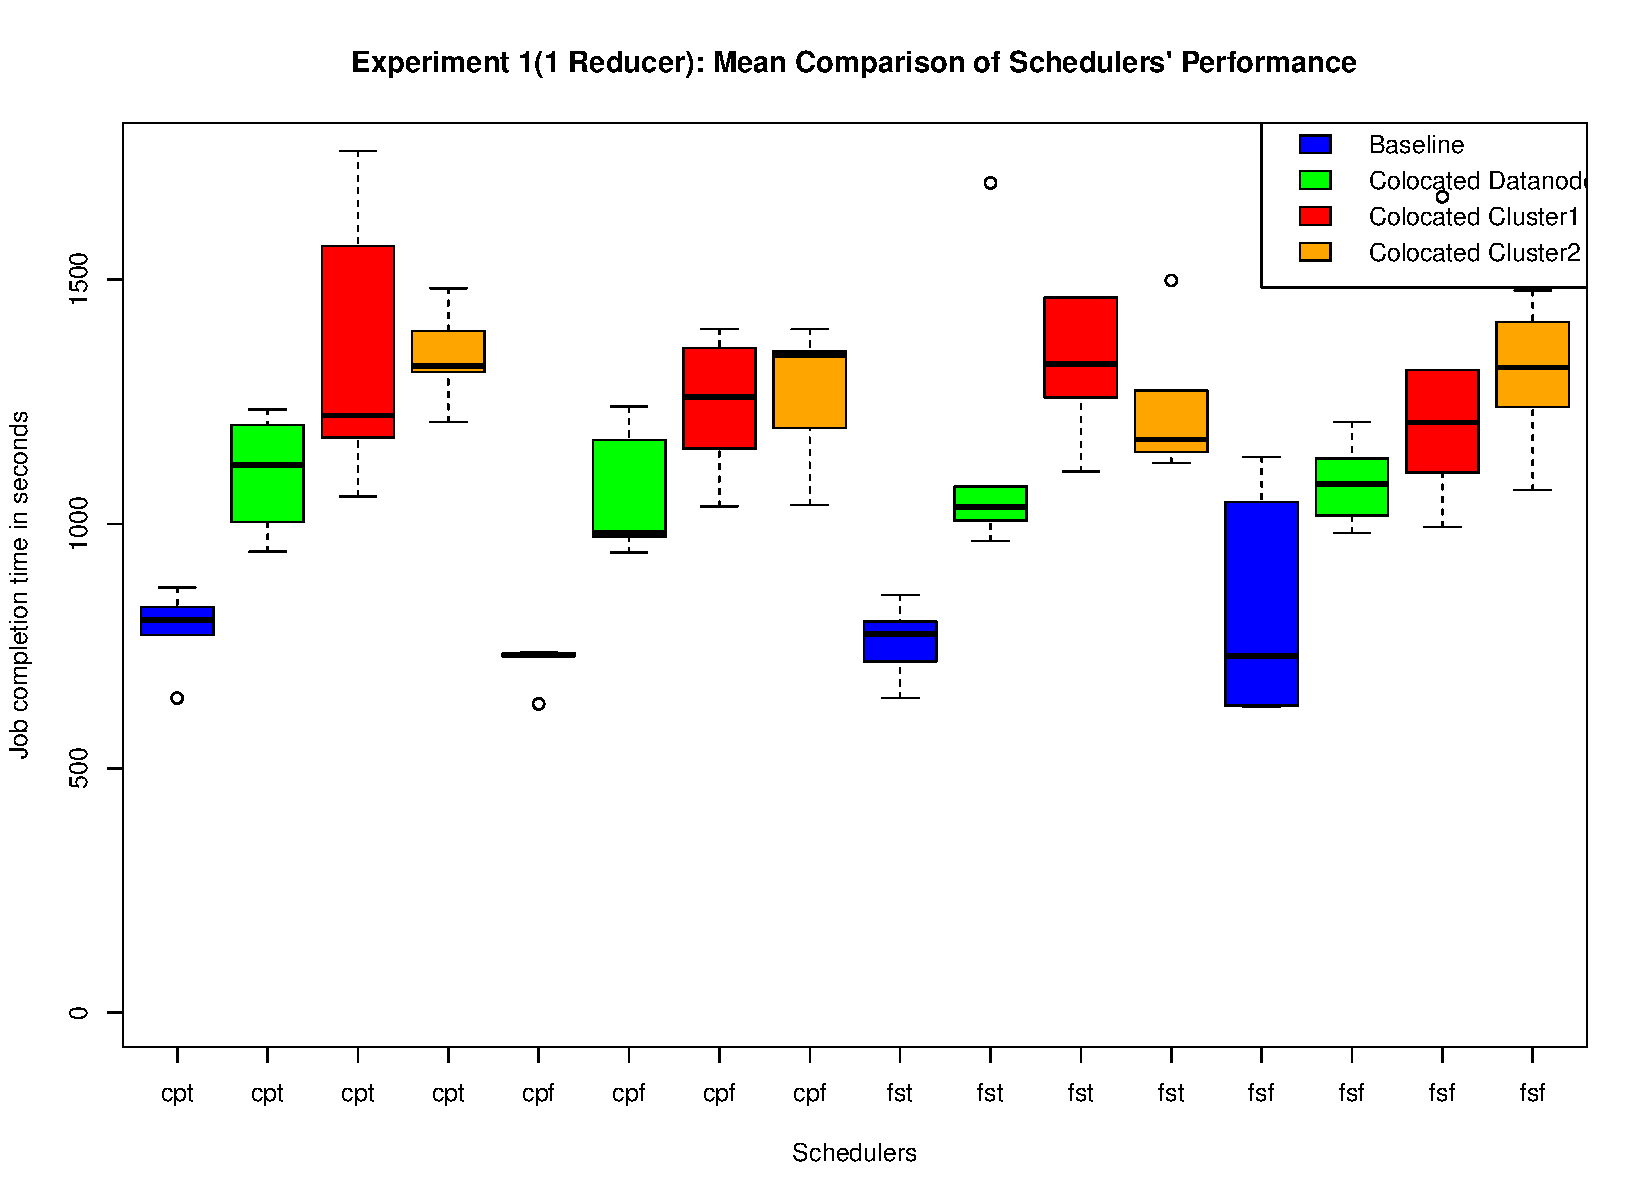
\includegraphics[width=\textwidth,height=\textheight,keepaspectratio]{./Figures/exp_1_mean.pdf}
    \rule{35em}{0.5pt}
  \caption{Experiment 1: Mean values of schedulers' performance }
  \label{fig:exp_1_mean}
\end{figure} 


\textbf{Capacity Scheduler with Speculative Task Execution (cpt)} For "cpt", the mean values of job completion time is around 850 seconds in baseline with distribution values for job completion time (performance variance) in range of 820 to 880 seconds. The mean value increases for the case of collocated datanodes to approximately 1125 seconds on average, and performance variance interval of 1000 to 1250 seconds. The collocated cluster case has the highest values for job completion ranging from 1200 to 1600 seconds with mean value of around 1400 seconds for cluster1, and range of 1340 to 1420 seconds with average of 1380 seconds for cluster2. The time difference of "cpt" performance between baseline and collocated datanodes case is 275 seconds, while the difference between baseline and collocated clusters case is higher with value of around 550 seconds.\\  

\textbf{Capacity Scheduler without Speculative Execution (cpf)} For "cpf" the mean values of scheduler performance is around 720 seconds with very small range performance variance. The collocated datanodes has the second best value for this scheduler with an average of 1125 seconds, and range of 1000 to 1250 seconds. The performance of scheduler for collocated cluster1 has an mean value of 1300 with range of 1200 to 1400 seconds, where for collocated cluster2 performance has mean value of 1310 seconds with range of 1220 to 1400 seconds. The time difference between baseline and collocated datanodes case is 405 seconds, while the collocated clusters have higher difference of 585 seconds.\\   


\textbf{Fairshare Scheduler with Speculative Execution (fst)} The "fst" scheduler has performance mean value of around 800 with range of values from 720 to 880 seconds. The collocated datanodes case has performance mean value of 1085 seconds, with range of 1050 to 1120 seconds. The performance of collocated cluster1 has mean value of 1400 seconds with range of 1320 to 1480 seconds. The performance of collocated cluster2 has mean value of around 1265 seconds with range of 1200 to 1330 seconds. The performance difference between baseline and collocated datanodes case is 285 seconds, and between baseline and collocated clusters case the difference is 630 seconds.\\ 

\textbf{Fairshare Scheduler without Speculative Execution (fsf) } The performance of "fsf" scheduler  has mean value of around 890 and range of values from 700 to 1080 seconds. The performance of "fsf" in collocated datanodes case has mean value of 1100 seconds, with range of 1020 to 1160 seconds. The "fsf" performance for collocated cluster1 has mean value of 1240 seconds for and range of values from 1120 to 1360 seconds. The "fsf" performance in collocated cluster2 case has mean value of around 1345 seconds with range of 1260 to 1430 seconds. The performance difference between baseline and collocated datanodes  case is 110 seconds, and between baseline and collocated clusters case the difference is 400 seconds.\\


\textbf{Side-Effects of Collocation} For three various node placement cases, the performance of both capacity scheduler and fairshare scheduler including the cases with and without speculative task execution are affected by collocation of datanodes. The results show that, collocation of datanodes has negative impact on performance of Hadoop schedulers and leads to longer job completion time. Though, in both collocation cases two datanodes were placed on single physical machine, but the collocated clusters case has worse results for Hadoop performance in comparison to collocated datanodes case. This is because in collocated clusters, the two nodes running on top of single machine are managed by two different namenodes, which does not know about each other, and their decisions harms the performance of collocated datanodes. It means, collocation of datanodes from different clusters does provide equal result to collocation of datanodes from the same cluster. \\  

\textbf{Speculation Effects }  For experiment one,  the speculative task execution does not improve the performance of Hadoop schedulers. Inversely, in baseline case for capacity scheduler the "cpf"‌ has better performance with mean value of 720 seconds in comparison to "cpt" which has mean value of 850 seconds. For fairshare scheduler, the "fst" has better performance compare to "fsf", in baseline,collocated datanodes and collocated clusters cases. As result for experiment 1,  the fairshare scheduler performance is improved using speculative task execution, while the capacity scheduler performance degraded by use of speculative task execution.   





\subsection{Fairness }

The figure \ref{fig:exp_1_max-min} illustrates the fairness of job completion time for all the schedulers. The figure \ref{fig:exp_1_max-min} shows that "fst" scheduler has the smallest range of values for job completion time in comparison to all other schedulers in baseline. For collocated datanodes and collocated clusters cases, the results of fairness is not well distinguishable, this is because, the number of reducers used in this experiment is only one, which means, results of the mappers should wait for single reducer for further process, thus, fairness is lost for almost all the cases of schedulers and placement cases.    

 \begin{figure}[htbp]
  \centering
    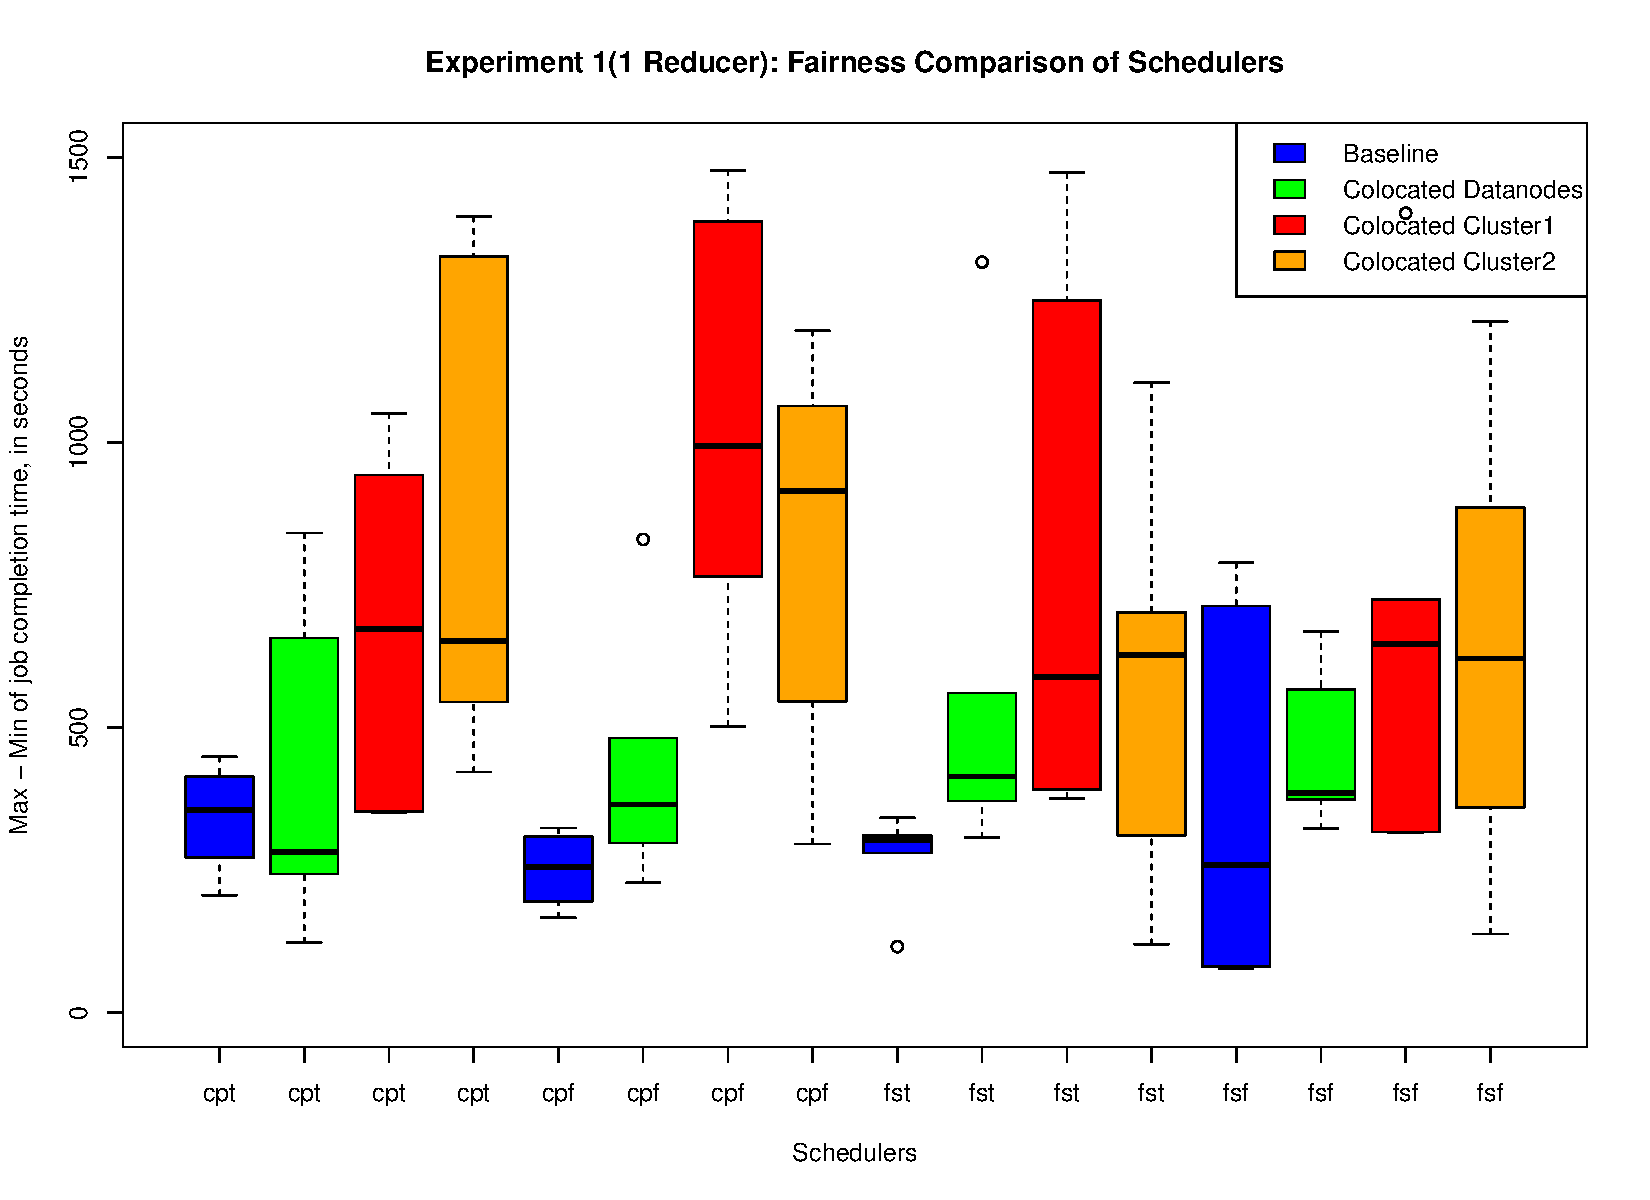
\includegraphics[width=\textwidth,height=\textheight,keepaspectratio]{./Figures/exp_1_max-min.pdf}
    \rule{35em}{0.5pt}
  \caption{Experiment 1: Fairness comparison of schedulers' performance }
  \label{fig:exp_1_max-min}
\end{figure} 
  

\subsection{Discussion}

There is single reducer used by terasort to complete the sort function for all mappers. If the reducer is used to process the output of a mapper, the output of other mappers should wait till the reducer become free. Waiting for reducer to redirect the output of mapper causes noticeable delay on performance of Hadoop schedulers. Thus, the results of experiment one, does not reflect clear distinguishable different values for the performance of capacity and fairshare schedulers. The philosophy behind fairshare scheduler is to provide fairness for all the jobs submitted.  The delay caused by single reducer to process output of mappers causes that, fairshare scheduler also does not have very vivid fairness in experiment one. The performance of schedulers for cases of speculative task execution and non speculative task execution are also affected almost equally by single reducer, thus, it makes it hard to judge from results of experiment one, that speculation leads to better performance of Hadoop scheduler. \\ 

The results explained for experiment one shows that, the collocation of datanodes either from same or different clusters leads to longer job completion time or performance degradation of Hadoop. Running two datanodes from the same cluster ( collocated datanodes case)‌ has better performance in compare to two datanodes from different clusters. It means, the side effects of a datanodes from different clusters is higher than side effects of datanodes from same cluster, and this is true for all the schedulers. \\  
  




 


%-----------------------------------
%	SUBSECTION 1
%-----------------------------------
\section{Experiment 2}

In experiment 2, single user submits five jobs to schedulers in all sub cases of experiment. Each job consists five GB‌ of data generated by Teragen (total of 25 GB data) and need to be sorted by terasort using Hadoop. Three copy of data were replicated and stored using HDFS‌ across datanodes of Hadoop cluster. There is no queue configuration for Hadoop schedulers and default root queue is  used for submission of all jobs. We changed (in contrast to experiment 1) the settings of experiment two and configured 10 reducers to participate in data processing. ‌ 




\subsection{Objectives}

As explained in discussion part of experiment one, single reducer causes considerable delay in job completion time for all Hadoop schedulers. The objective of experiment 2 is to see how the number of reducers has affect on job completion time or performance of Hadoop. In experiment two, by increasing the number of reducers to ten, our expectation was to have better performance evaluation in comparison to experiment one. It is also important, to see how the performance of Hadoop is improved by increased number of reducers for collocated datanodes and collocated clusters. 



\subsection{Results}
The figure \ref{fig:exp_2_mean} illustrates the mean value results for all the experiment cases. Over all , the job completion time is better than experiment one, it means number of reducers have important role in Hadoop performance.\\

\begin{figure}[htbp]
  \centering
    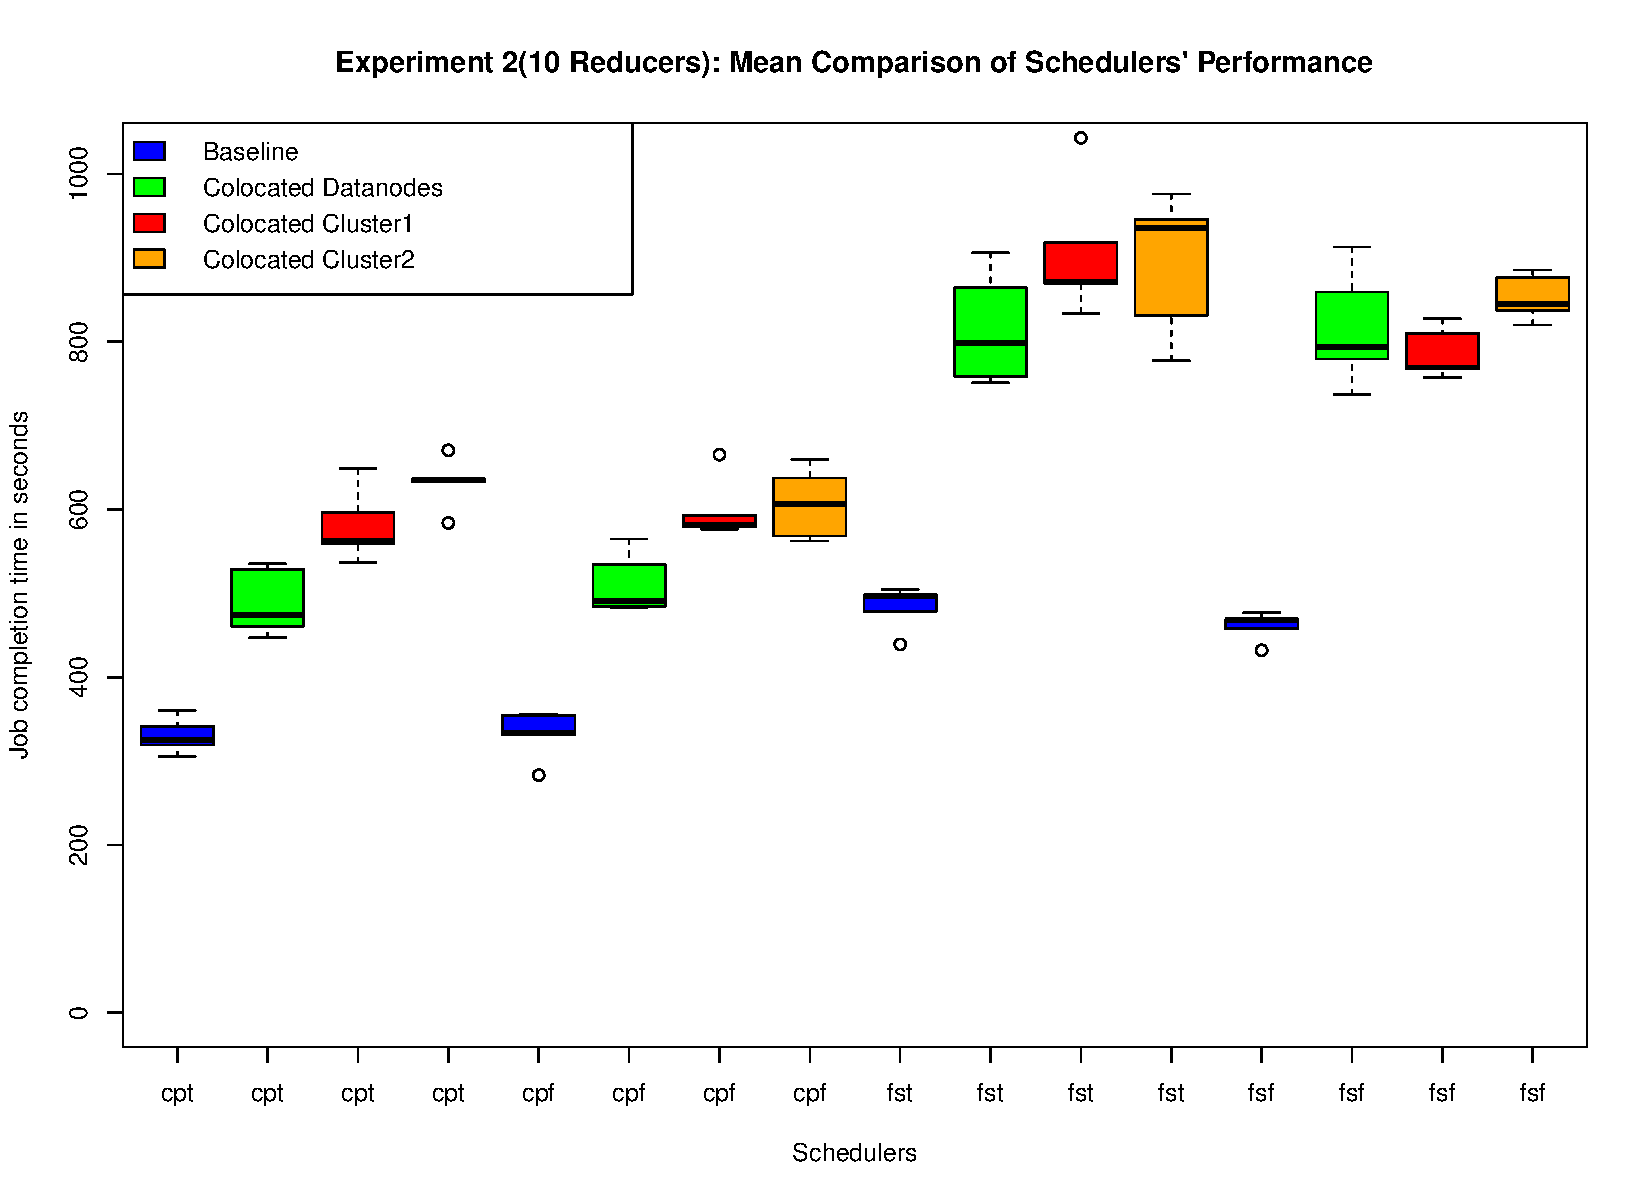
\includegraphics[width=\textwidth,height=\textheight,keepaspectratio]{./Figures/exp_2_mean.pdf}
    \rule{35em}{0.5pt}
  \caption{Mean value of schedulers' performance }
  \label{fig:exp_2_mean}
\end{figure} 

\textbf{Capacity Scheduler with Speculative Execution (cpt)} The mean value for "cpt" performance in baseline case is approximately 300 seconds, which is the best value among all schedulers cases. For collocated datanodes, the scheduler performance has mean value of approximately 500 seconds, which shows that collocation of datanodes increased the job completion time 70\% more than the baseline. For collocated clusters cases, the scheduler performance has mean value of approximately 600 seconds (approximate average for both clusters), which is double value of job completion time in comparison to baseline and shows 100\% increment job completion time.\\

\textbf{Capacity Scheduler without Speculative Execution (cpf)}  The mean value for "cpf" performance  in baseline case is approximately 330 seconds, which is worse than "cpt" ( which was 300 seconds), but the second best result among all the schedulers. The side effects for collocated datanodes case of "cpf" is almost similar to "cpt". The collocation of datanodes has an average performance of approximately 530 seconds for job completion time, which shows 70\% increment in job completion time in comparison to baseline. The average performance for collocated clusters is approximately 600 seconds for both clusters, which shows 95\% increment in job completion time. \\


\textbf{Fairshare Scheduler with Speculative Execution (fst)} The mean value for "fst" performance in  baseline case is approximately 500 seconds, which is the worst mean value among all schedulers' performance. The "fst" performance in collocated datanodes case has mean value of around 800 seconds, which shows 60\% increment and time difference of 300 seconds for job completion time in comparison to baseline. The "fst" performance in collocation of datanodes case from different Hadoop clusters has mean value of around 900 seconds, which shows 80\% increment (400 seconds time difference of job completion time) in comparison to baseline case.\\

\textbf{Fairshare Scheduler without Speculative Execution (fsf) } The  mean value for "fsf" performance  in baseline case is approximately 480 seconds, which is better than "fst" and third best value among all the schedulers. The "fsf" performance in collocation of datanodes case has mean value of approximately 800 seconds for job completion time, which shows 66\% increment and 320 seconds time different in comparison to baseline case. The "fsf" performance in collocated datanodes case from different clusters,  has mean value of around 800 seconds ( approximate value for both clusters), which is the same result as collocated datanodes case in comparison to baseline. \\


\textbf{Side-Effects of Collocations } To analyse the side effects of datanodes collocation and clusters collocation, we categorise the schedulers to capacity share scheduler and fairshare scheduler. The results in figure \ref{fig:exp_2_mean} shows, that fairshare scheduler has worse performance for the collocation cases in comparison to capacity share scheduler. The mean value difference between baseline and collocated datanodes for "fst", which shows the side effects of collocation is around 300 seconds, while this value is around 200 seconds for "cpt" case. Also, the mean value difference between baseline and collocated clusters cases, for "fst" it is 400 seconds, while this value is 300 seconds in "cpt" case.\\ 

For cases, where tasks are executed by schedulers without speculation (like "cpf" and "fsf" cases), still , capacity share scheduler has better performance for collocation cases in comparison to fairshare scheduler. The mean value difference for between baseline and collocated datanodes for "cpf" is 200 seconds, which is better than the mean value difference of 320 seconds for "fsf" case. The mean value difference between baseline and collocated clusters cases for "cpf" is 270 seconds, for which "fsf" has higher difference of 320 seconds. 


\textbf{Speculation Effects } By having a deeper look to mean values in figure \ref{fig:exp_2_mean}, it is obvious that speculative task execution improved the performance of capacity share scheduler ( see the "cpt" case), while decreased the performance of fairshare scheduler. Though the performance improvement of speculative task execution is minor, but still the improvement for "cpt"‌ is consistent and true for the collocated cases in comparison to "cpf" case. In opposition to capacity share scheduler, the  fairshare scheduler with speculative task execution, in "fst" case has worse result in comparison to "fsf" case. \\  ‌  


 \subsection{Fairness}
 The figure \ref{fig:exp_2_max-min} illustrates the fairness for job completion time, among submitted jobs for each placement and schedulers cases. The results show that overall fairshare scheduler has much better fairness in comparison to capacity share scheduler. The fairness for job completion time ranges from around 50 to 200 seconds for all the placement cases of fairshare scheduler, while the results for capacity share scheduler ranges from 200 to 400 seconds.\\ 
 
 
 
  For "cpt" in baseline case, the fairness values for job completion time is in the interval of 210 to 260 seconds, which shows at least 210 seconds difference. While for both "cpt" and "cpf" in baseline case, the fairness values is lower than 300 seconds on average, the collocation had negative impact and increases the fairness values to higher than 300 seconds, and even close to 400 seconds for collocated datanodes case of "cpt".
 
 
 \begin{figure}[htbp]
  \centering
    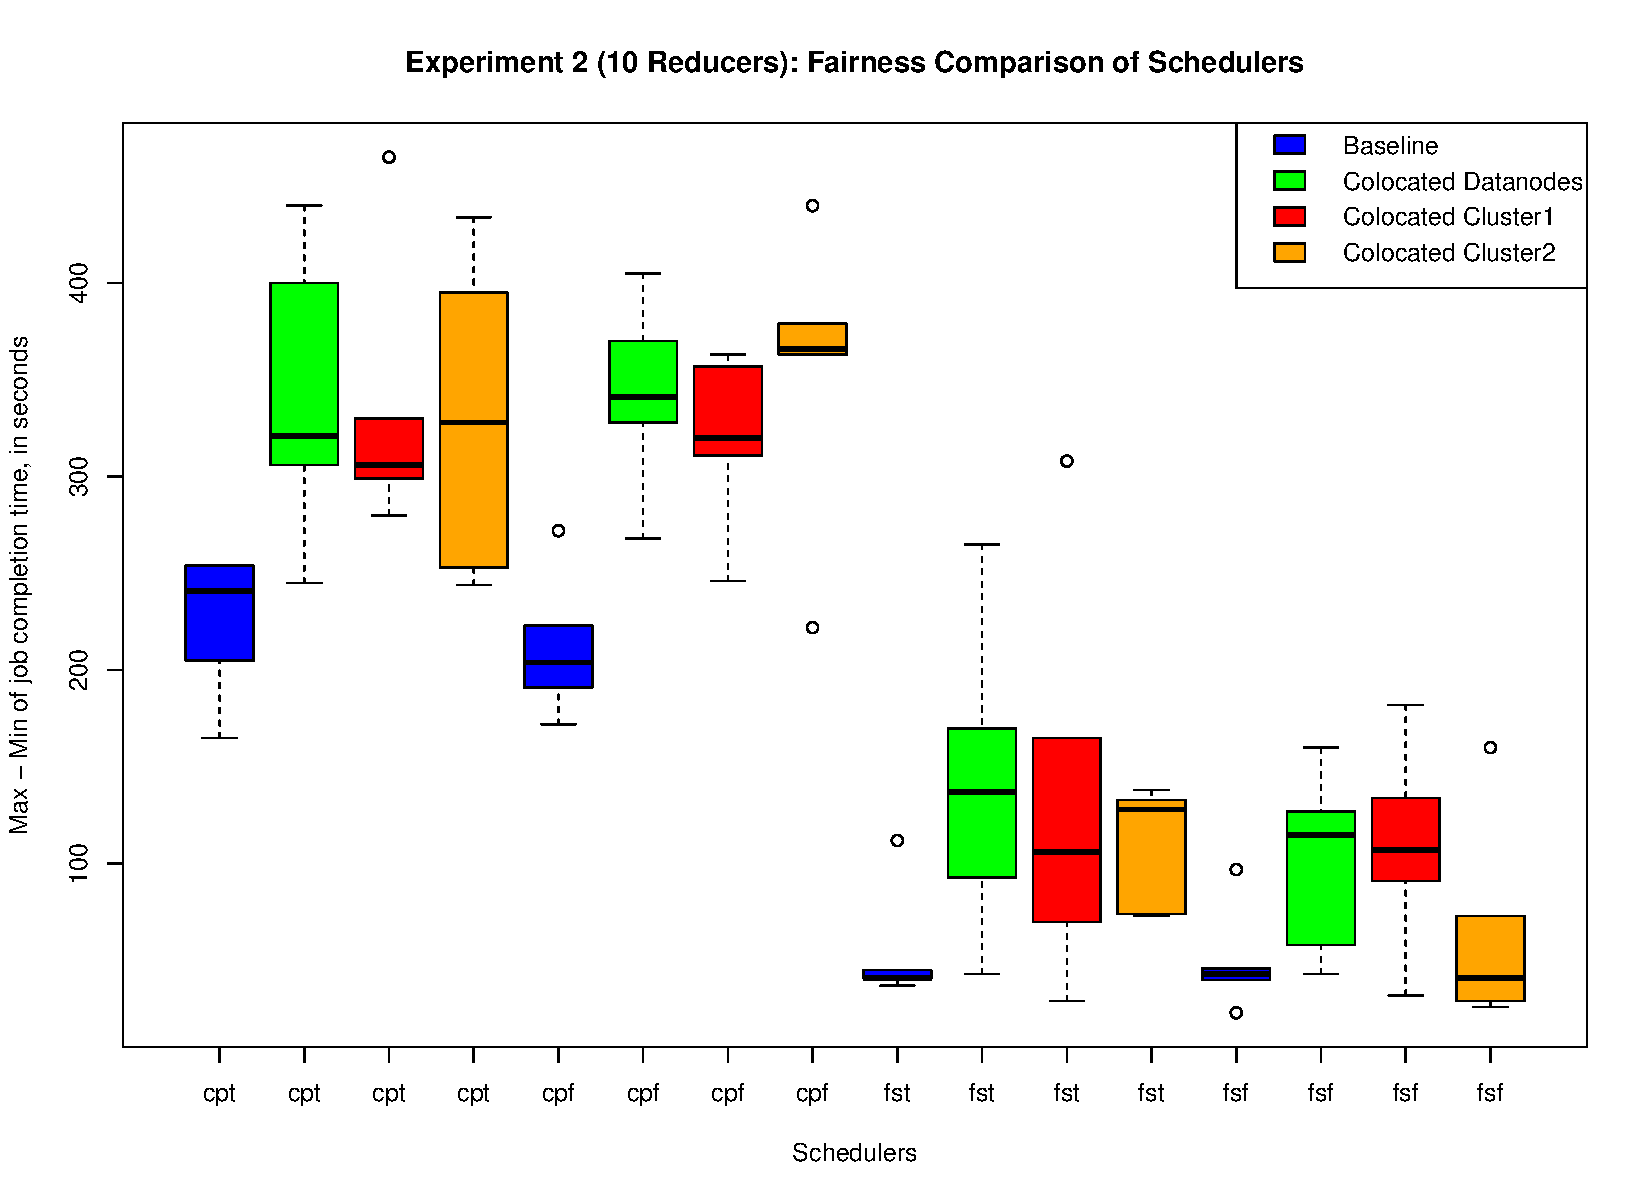
\includegraphics[width=\textwidth,height=\textheight,keepaspectratio]{./Figures/exp_2_max-min.pdf}
    \rule{35em}{0.5pt}
  \caption{Experiment 2: Fairness comparison of schedulers' performance }
  \label{fig:exp_2_max-min}
\end{figure} 
  

\subsection{Discussion}

By increasing the number of reducers from one ( in experiment one) to ten ( in experiment two ), we see that the performance of Hadoop schedulers are improved for all the cases. Which means, for process of workload using Hadoop, the selection of fair number of reducers plays key role on over all performance of Hadoop. The number of mappers were consistent for all the schedulers, it was 40+ mappers. In case of speculation cases of schedulers, some tasks were speculatively executed, which added speculative number of mappers and reducers. \\


The results shown for experiment two, indicates that capacity share scheduler has better performance in comparison to fairshare scheduler, and executes the submitted jobs in smaller time interval than fairshare schedulers. The performance of capacity share schedulers is better than fairshare schedulers in both cases of speculative and non speculative task execution, and all collocation cases.\\

The collocation cases have impact on schedulers performance and degrades the performance of Hadoop schedulers. The side effects of collocation for fairshare schedulers are higher than capacity share. The side effects of collocated datanodes is not as much as collocated clusters. This is because, in collocated datanodes, both nodes are controlled by single namenode,which mean, namenode is aware of the status of namenode using resources manager. In collocated clusters cases, the collocated datanodes are belong to separate namenodes that are not aware of status of collocated datanode, so the performance of datanode from cluster one, effects the performance of datanode of cluster two.\\  
 

 The fairshare schedulers provide better fairness performance for submitted jobs. Considering the performance evaluation of and fairness evaluation of schedulers, the fairness has cost for fairshare schedulers and that causes performance degradation of Hadoop. One may use capacity share to have better performance and fairshare scheduler to guarantee better fairness for job process.\\



%-----------------------------------
%	SUBSECTION 2
%-----------------------------------

\section{Experiment 3}
The results from experiment two shown that increasing the number of reducers improves the performance of Hadoop. In experiment three, we increased the number of reducer to twenty (20) reducers, which is 50\% of the number of used mappers. Rest of the experiment settings were the same as experiment one and two, where single users submitted five jobs, each job consist of five GB of data. There were no special queue configuration for Hadoop schedulers. The experiment was executed for all the placement cases and schedulers cases. 
  
\subsection{Objective}
The objective of the experiment was to find out the effects of increased number of reducers on performance of Hadoop schedulers. The side-effects of collocation and evaluation of performance improvement for the schedulers were the other objectives. The improvement of fairness for schedulers and  performance improvement of schedulers by speculative task execution were the other expected outcome of the experiment. 

\subsection{Results }
By increasing the number of reducers to 20 reducers, the evaluation shows that performance of Hadoop is optimized across all the schedulers. While the effect of changing the number of reducer for experiment to experiment two was very vivid and clear, the effect of changing the number of reducers from ten to twenty in experiment three is not so high in comparison to experiment two. This means, that having so many reducers does not improve the performance of Hadoop and we may select a fair number schedulers for Hadoop. The figure \ref{fig:exp_3_mean} illustrates the mean values for schedulers in all the placement cases.  


\begin{figure}[htbp]
  \centering
    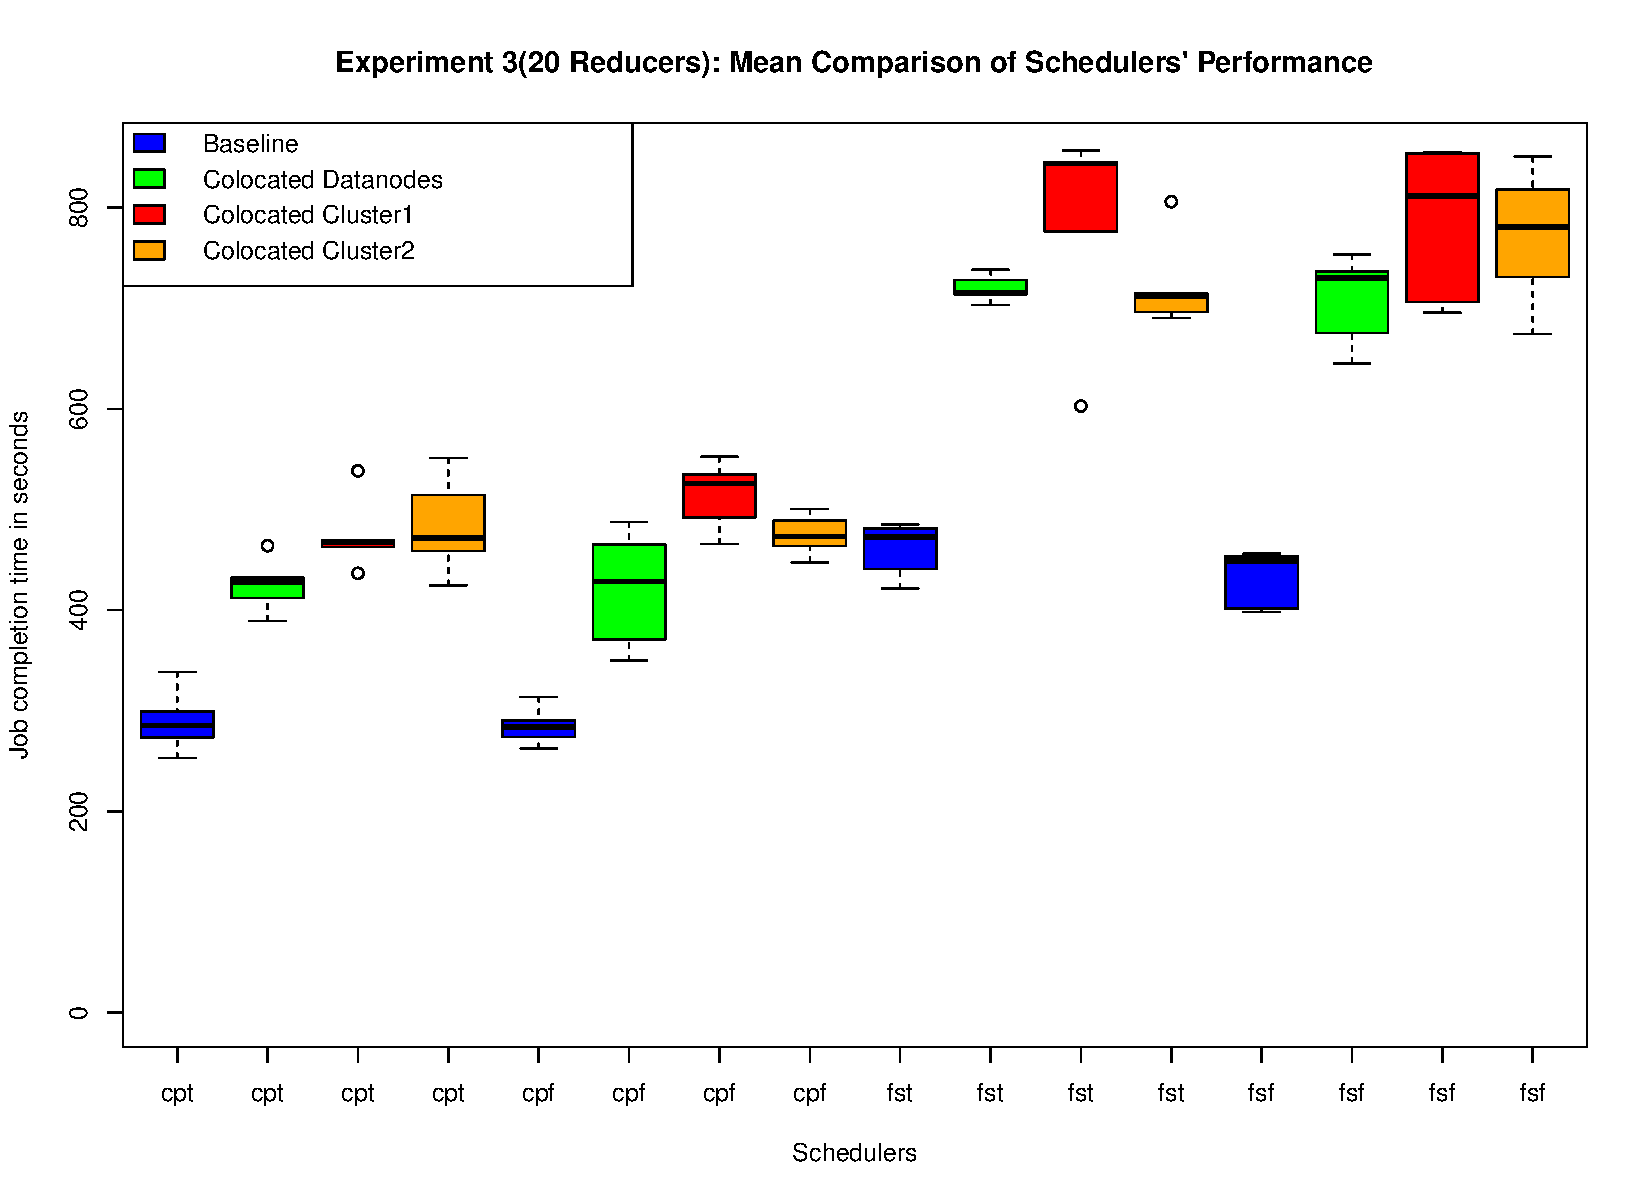
\includegraphics[width=\textwidth,height=\textheight,keepaspectratio]{./Figures/exp_3_mean.pdf}
    \rule{35em}{0.5pt}
  \caption{Experiment 3: Mean value of schedulers' performance}
  \label{fig:exp_3_mean}
\end{figure}


\textbf{Capacity Scheduler with Speculative Execution (cpt)} The mean value for "cpt" performance in baseline case is approximately 290 seconds. For collocated datanodes, the scheduler has mean value of approximately 420 seconds for job completion time, which shows that collocation of datanodes increased the job completion time 45\% more than the baseline. For collocated clusters case, the scheduler has job completion time of approximately 500 seconds (approximate average for both clusters), which has time difference of 210 seconds in comparison to baseline and shows 72\% increment in job completion time.\\

\textbf{Capacity Scheduler without Speculative Execution (cpf)} The mean value for "cpf" performance  in baseline case is approximately 290 seconds, which is same as "cpt", but the distribution range of job completion time is smaller in comparison to "cpt" . The side effects of datanodes collocation case on "cpf" is almost similar to "cpt", but the job completion time is scattered in larger interval of time. The collocation of datanodes has an average of approximately 430 seconds for job completion time, which shows 48\% increment in job completion time in comparison to baseline. The average job completion time for collocated clusters is approximately 520 seconds for both clusters, which shows 79\% increment in job completion time. \\ 


\textbf{Fairshare Scheduler with Speculative Execution (fst)} The mean value for "fst" performance in  baseline case is approximately 470 seconds, which is the worst mean value among all schedulers' performance in baseline. The collocated datanodes, has performance with mean value of around 710 seconds, which shows around 51\% increment and time difference of 240 seconds for job completion time in comparison to baseline. The collocation of datanodes from different Hadoop clusters are very different, cluster1 has a mean value of around 800 seconds, and cluster2 has mean value of 700 seconds. The mean value for both clusters is around 750 seconds,  which shows around 60\% increment with 280 seconds time difference of job completion time in comparison to baseline.\\

\textbf{Fairshare Scheduler without Speculative Execution (fsf) } The  mean value for "fsf" performance  in baseline case is approximately 430 seconds, which is better than "fst" and third best value among all schedulers. The collocation of datanodes, has mean value of approximately 700 seconds for job completion time, which shows around 63\% increment and 270 seconds time different in comparison to baseline. The collocated datanodes from different clusters have mean value of around 750 seconds ( approximate value for both clusters), which shows around 74\% increment with time difference of 320 seconds for job completion time in comparison to baseline. \\
 ‌  
\textbf{Node Placement Effects } Similar to experiment two, the side effects of collocation for both collocated datanodes and collocated cluster cases is high for fairshare scheduler in comparison to capacity share scheduler. For capacity schedulers the mean value of baseline in comparison to collocated datanodes and collocated clusters cases show the respectively time difference values of 135 and 220 seconds. While, for similar comparison the fairshare schedulers have time difference values of 255 and 300 seconds. \\    

 Across all the schedulers, the mean values for collocated datanodes is lower than mean value for collocated clusters. This proofs the fact, that collocation of datanodes from same cluster has less side effects on collocated datanode in comparison to collocation of datanodes from different schedulers.\\  



\textbf{Speculation Effects }  The illustrated results in figure \ref{fig:exp_3_mean} shows that the speculative task execution does not improve the performance of schedulers in all the cases. For "fst" in baseline case, the speculative task execution leads to worst result in comparison to "fsf". The comparison of mean values for "cpt" and "cpf" shows that there are no vivid performance improvement between speculative and non speculative task execution in all the placement cases. \\ 

 

\subsection{Fairness}
 The figure \ref{fig:exp_3_max-min} illustrates the fairness for job completion time, among submitted jobs for each placement and scheduler cases. As the results show, the fairshare schedulers have  values  lower than 250 seconds, in contrast , the fairness values for capacity share schedulers are higher than 250 seconds. The "fsf" scheduler has the best fairness value of 50 seconds, with small range of of distribution for job completion time. The fairness values shown for fairshare schedulers in collocated cases indicates that, collocation of datanodes has negative impact on fairness of schedulers, and leads to larger range for job completion time.\\ 
 
 The results shown for capacity share schedulers in all the placement cases explains, that they have higher value of 250 to 500 seconds. Both collocation cases (collocated datanodes and collocated clusters) have almost similar fairness values with mean of around 450 seconds for almost both "cpt" and "cpf", while "cpf" has larger range values for job completion time.  
 
 
  

\begin{figure}[htbp]
  \centering
    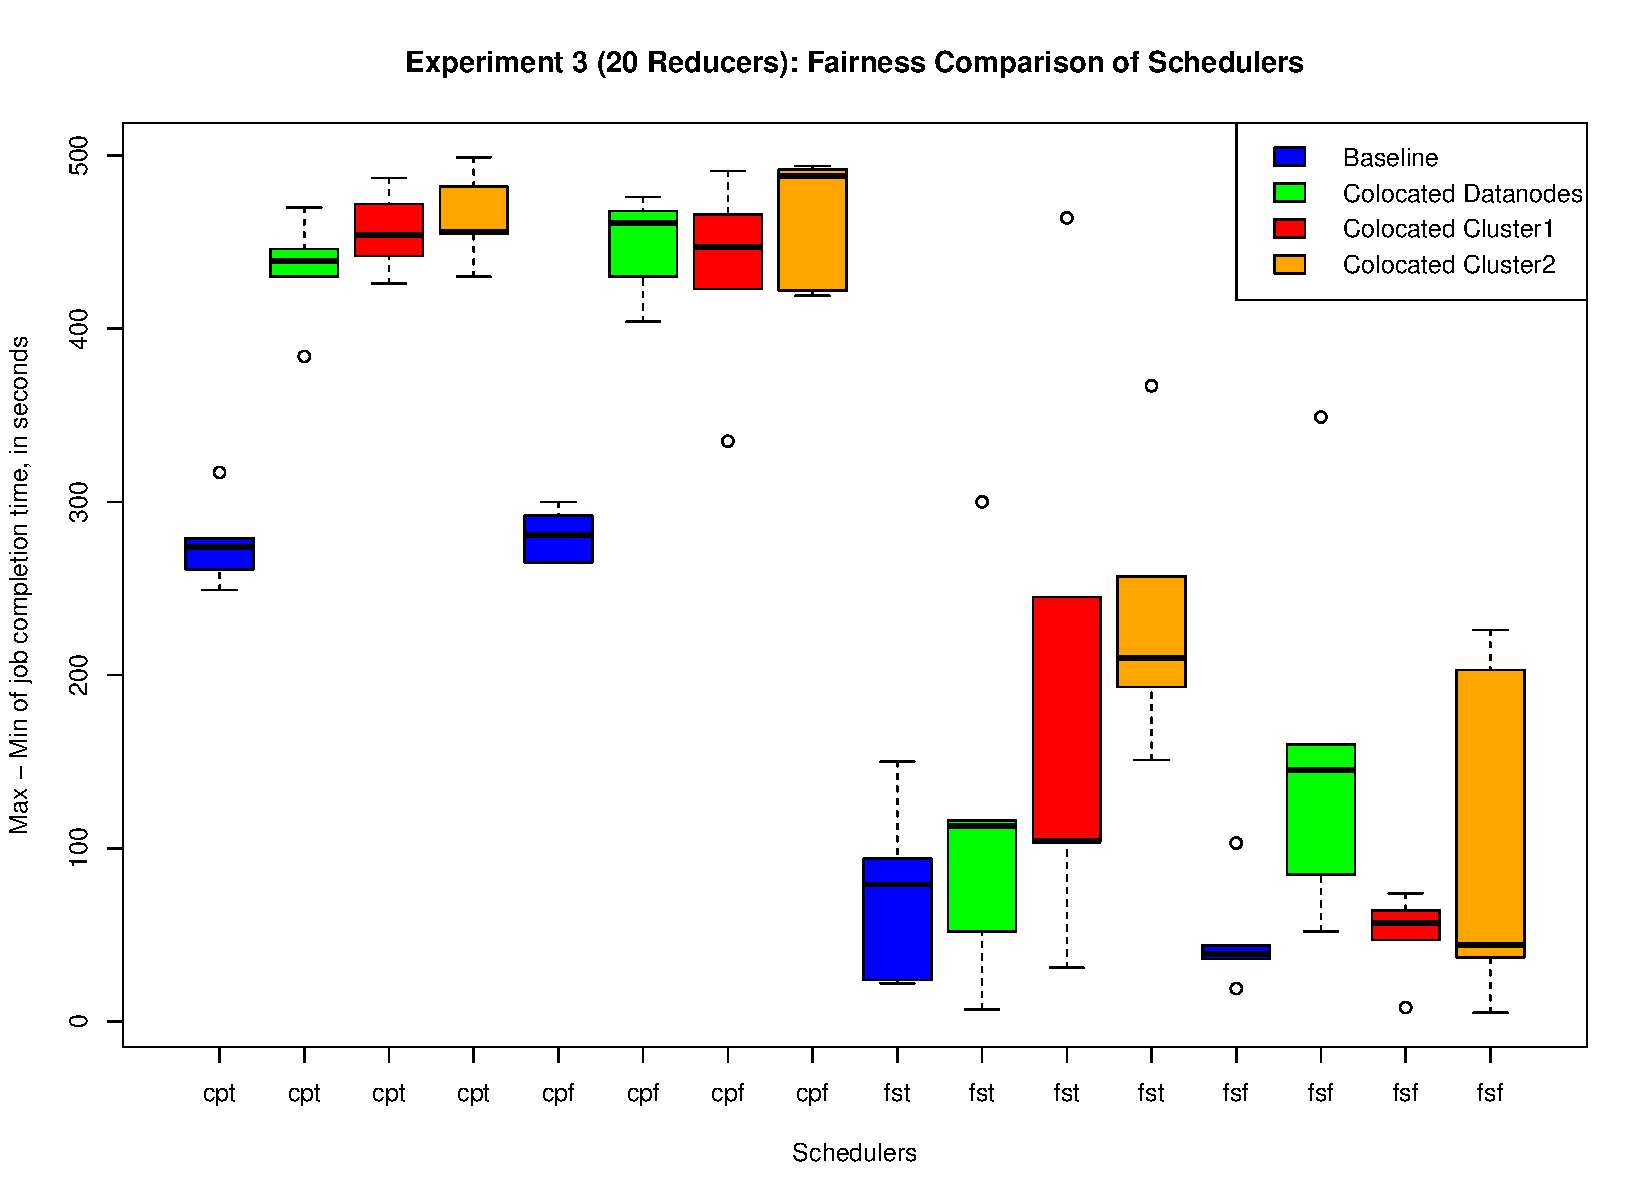
\includegraphics[width=\textwidth,height=\textheight,keepaspectratio]{./Figures/exp_3_max-min.pdf}
    \rule{35em}{0.5pt}
  \caption{Experiment 3: Fairness comparison of schedulers' performance }
  \label{fig:exp_3_max-min}
\end{figure}

\subsection{Discussion}
Though increasing the number of reducer lead to better performance in experiment two, in experiment three by increasing the number of reducers to twenty, which is 50\% of mappers (total of 40 mappers were used), the performance improvement is not so much. It means, selection of high number of reducers does not improve the performance of Hadoop, and we must select a fair number of reducers. The results from all three experiments (experiment one, two and three) for which the number of reducers were respectively 2.5\%, 25\% and 50\% of mappers, the experiment three had best results for all the schedulers in all the cases.\\


In regard to performance evaluation of schedulers, in one hand, the capacity share scheduler has the best results for both "cpt" and "cpf" cases. on the other hand, the capacity scheduler has worst fairness results in comparison to fairshare scheduler. Inversely, the fairshare scheduler has the worst performance for job completion and best fairness values in comparison to capacity share scheduler. \\

Similar to two previous experiments, the collocation cases have negative impact on performance of schedulers. In comparison to fairshare scheduler, the capacity share scheduler has more tolerance to collocation of datanodes in both cases of collocated datanodes and collocated clusters and has better performance. The capacity share scheduler also have minor better performance while speculatively executing the tasks, while in fairshare scheduler the speculative task execution causes minor degradation to the performance of scheduler.  \\  
 

 


%----------------------------------------------------------------------------------------
%	SECTION 2
%----------------------------------------------------------------------------------------

 
% Chapter Template

\chapter{Cloud Computing in Afghanistan} % Main chapter title

\label{Chapter6} % Change X to a consecutive number; for referencing this chapter elsewhere, use \ref{ChapterX}

\lhead{Chapter 6. \emph{Cloud Computing in Afghanistan}} % Change X to a consecutive number; this is for the header on each page - perhaps a shortened title

%----------------------------------------------------------------------------------------
%	SECTION 1
%----------------------------------------------------------------------------------------
Afghanistan is land lock country which most parts are enclosed by mountains. In the last two decades (80s and 90s), socio-political upheavals and war not only destroyed Afghanistan’s infrastructures and wealth, but it also destroyed the Information and Communication Technology (ICT) systems. Large  number of Afghan people scattered in and out of Afghanistan during last three decades of war.  This made the ICT services and facilities an essential issue for Afghanistan’s immediate reconstruction. After the Temporary Government in 2001 established in Afghanistan, the country obtained new view of political and socio-economic rehabilitation and structure. 

\section{Afghanistan and ICT}
 
  By establishment of the new government after 2011, Afghan government started to encourage the private sector to do investment in Afghanistan's ICT projects. Parallel to the investment of private sectors on ICT field  the government also started to develop ICT infrastructure and services in Afghanistan. As result of encourages big investors like Afghan Wireless Company (AWCC), Roshan, Areeba and Etisalat entered to ICT market of Afghanistan. In order to develop ICT and to fulfil the human resource requirements of the ICT field in Afghanistan the Afghan government Established Computer Science Faculties in many universities of Afghanistan, ICTI institute , creation of ICT Law and ICT strategy plan. Almost 80 percent of Afghan people have access to telecommunication that indicates rapid growth of ICT and implementation of ICT projects. In this section our focus is more on national projects which are offered or going to be offered by Afghan government.\cite{afg1}\\

Afghan people need to strengthen and diversify their economies, educate and engage their young people, develop the infrastructures that support economic growth, and lure back the educated professionals and business-people who have fled to other countries. ICT will be instrumental in meeting these challenges, but recent history shows that Afghanistan is suspicious of, and resistant to, technological change. Based on a report by the United Nations Science and Technology Group for Development (UNSTD), ICT strategies are often developed and publicized mainly to attract external investment to construct new infrastructures or to market hardware and software without giving sufficient attention to local concerns and requirements \cite{afg2}.\\


\subsection{National Optical Fiber Backbone}
This project will install a national backbone network across the country, which will support all the other projects (digital lines, microwave, etc). It will allow a high volume of national and international traffic and will connect major provinces and to neighbouring countries. This Network will link many of the principle cities of Afghanistan following the route of the national roadway system. This project is for the turnkey construction and operation of the complete Optical Fiber Communication (OFC) ring around Afghanistan which is estimated approximately 3.200 km length. In addition to linking many of the key cities. This project also calls for the construction of accesses to the backbone for the other cities and provinces not directly on the backbone route. Those access routes for the other cities and provinces will be taken up separately. There will be other major spurs off this main loop connecting to neighbouring countries Iran, Pakistan, Uzbekistan, Tajikistan, and Turkmenistan.\cite{afg1} 	


\section{Challenges}
Although, Afghan ICT had good progress in past years, but still there are challenges that needs time to be solved. Low levels of education and literacy, poor IT infrastructures, lack of ICT skilled human resources, lack of political interest to ICT can be counted as number of challenges. Security is a big challenge that not only ICT project implementation but over all Afghan government suffer from.  Lack of skilled human resources is another challenge, even use of the Internet requires a fairly complex set of skills and technology, at very least, one must have electricity, a communications line, a terminal capable of interacting across the communications lines, and (in most cases) a reasonable fluency in English \cite{afg3}. 


\section{Cloud Computing In Afghanistan}

The telecommunication companies currently launched 3G services, through which Afghan civilians can access Internet via cell phones. Considering that more than 80\% of the Afghan population has access to telecommunication services, launch of General Radio Packet Services (GPRS) and 3G services are major achievement for provision of Internet access to the civilians. For the organizations invested in ICT market of Afghanistan, poor IT infrastructure infrastructure, lack of security, required energy resources, IT experts all these challenges makes it difficult to establish and  maintain large data centres of their own for storage and process of their data. Still most of these companies use microwave of satellite links to connect to the Internet and very few and limited fibre links are available across the country as backbone links.\\

 The organization only need Internet connection with high enough speed to access the cloud services/infrastructure and use it according to their need. Using cloud services, the organizations are free of headache for maintenance, physical resources, security and hiring experts to manage IT resources. Though some of major ICT companies that have stable internet connection such as Roshan company rely on partial cloud service, but overall the poor infrastructure of ICT causes unstable Internet connections, which makes it difficult to even go for cloud services in Afghanistan. After completion of national projects in Afghanistan, such OFC‌ project  the organizations may have stable Internet connection that will ease the use and cultivation of cloud services among organization. The organizations may rely on cloud computing services where all the infrastructure, resources, storage, process and maintenance is provided by cloud operator to the clients via an Internet connection. \\
 
   
    
 


 
% Chapter Template

\chapter{Conclusion} % Main chapter title

\label{Chapter7} % Change X to a consecutive number; for referencing this chapter elsewhere, use \ref{ChapterX}

\lhead{Chapter 7. \emph{Conclusion}} % Change X to a consecutive number; this is for the header on each page - perhaps a shortened title

%----------------------------------------------------------------------------------------
%	SECTION 1
%----------------------------------------------------------------------------------------

\section{Conclusions}
 
 
 The experimental results explained in \ref{Chapter5} gives the idea that Hadoop optimizations does not improve the performance of Hadoop for every dataset process. For cloud services where physical computational resources are shared among multiple organizations to run Hadoop cluster(s), using capacity share scheduler of Hadoop is better choice in comparison to fairshare scheduler. Overall, the capacity scheduler of Hadoop has good performance in term of job completion time, but it has poor fairness results for job completion time. \\
 
 As the name explains, fairshare scheduler of Hadoop has better fairness in all the cases in comparison to capacity share scheduler of Hadoop, but it has poor performance than capacity share scheduler. For submitted jobs to Hadoop cluster from single or multiple organizations, in case fairness is important, than fairshare scheduler is better choice, otherwise , capacity scheduler has better performance. \\
 
 The collocation of more than one VM acting as datanode on top physical machine, degrades the performance  of Hadoop cluster. Collocation of VMs (datanodes)‌ from same cluster has better results in comparison to placement of VMs from different Hadoop clusters. Though the performance of Hadoop schedulers are degraded by collocation, but capacity share scheduler is more robust to collocation of datanodes.\\
 
 The thesis explored the analysis of speculative task executions by Hadoop schedulers. The speculative  

\section{Future Work}

%----------------------------------------------------------------------------------------
%	SECTION 2
%----------------------------------------------------------------------------------------



 


%----------------------------------------------------------------------------------------
%	BIBLIOGRAPHY
%----------------------------------------------------------------------------------------

\label{Bibliography}

\lhead{\emph{Bibliography}} % Change the page header to say "Bibliography"

\bibliographystyle{unsrtnat} % Use the "unsrtnat" BibTeX style for formatting the Bibliography

\bibliography{Bibliography} % The references (bibliography) information are stored in the file named "Bibliography.bib"

\backmatter
%----------------------------------------------------------------------------------------
%	THESIS CONTENT - APPENDICES
%----------------------------------------------------------------------------------------

\addtocontents{toc}{\vspace{2em}} % Add a gap in the Contents, for aesthetics

\appendix % Cue to tell LaTeX that the following 'chapters' are Appendices

% Include the appendices of the thesis as separate files from the Appendices folder
% Uncomment the lines as you write the Appendices

% Appendix A

\chapter{Appendix A} % Main appendix title

\label{Used Scripts} % For referencing this appendix elsewhere, use \ref{AppendixA}

\lhead{\emph{Appendix A}} % This is for the header on each page - perhaps a shortened 

The process of running experiments were automated using python scripts. This appendix contains the scripts used for experiment execution and log processing. Most of the scripts are written using "pyton" scripting language. For plotting the results, both "bash" and "R" scripts were used. The scripts were written in a joint work by me and my advisor Mr.Lalith Suresh. 


\section{Experiment Execution Scripts}
 Below Python scripts were used to install, configure and run Hadoop on experimental environment. 

\subsection{sideEffects Python Script}

\begin{verbatim}
#file name: side_effects.py
# This file was the main file to start the process of installation, configuration and running Hadoop.

from interact import *
from placement import *
from cassandra_utils import *
from resource_bench_utils import *
import hadoop_utils
import simplejson
import time
import glob
import os
import shutil
from common_monitors import *
from multiprocessing import Process

NODE_LIST = ["loadgen162", "loadgen163", "loadgen164", "loadgen165", 
            "loadgen166", "loadgen167", "loadgen168"]
def run_hadoop_baseline(pm, nodes_used, workload, schedule):
    ''' This is a single run to gather the baseline resource
        and performance profile for hadoop  '''

    ###### SPAWN VMS ##########
    hadoop_utils.spawn_hadoop_vms(pm["hadoop:num_hadoop"],
                     pm["exp_number"],
                     pm["hadoop:placement"])
    time.sleep(120)

    ####### START PROCESSES ##########

    hadoopStartProcess = Process(target=hadoop_utils.setup_hadoop, 
        args=(pm["hadoop:num_hadoop"],
     pm["exp_number"],pm, schedule))
    hadoopStartProcess.start()
    hadoopStartProcess.join()
    #time.sleep(120)

    ####### LOAD DATA ##########

    hadoopLoadProcess = Process(target=hadoop_utils.hadoop_load_workload, 
        args=(pm, pm["exp_number"], workload ))
    hadoopLoadProcess.start()
    hadoopLoadProcess.join()
    time.sleep(5)

    ####### RUN WORKLOAD ##########
    run_mpstat(nodes_used, pm["exp_number"])
    run_bwmon(nodes_used, pm["exp_number"])
    run_iostat(nodes_used, pm["exp_number"])
    hadoopRunProcess = Process(target=hadoop_utils.hadoop_run_workload, 
        args=(pm, pm["exp_number"], workload))
    #time.sleep(40)

    hadoopRunProcess.start()
    hadoopRunProcess.join()
    #time.sleep(180)
    retreive_mpstat_results(nodes_used, pm["exp_number"])
    retreive_bwmon_results(nodes_used, pm["exp_number"])
    retreive_iostat_results(nodes_used, pm["exp_number"])

def delete_hadoop_vms(num_hadoop,
                     exp_number,
                     placement_map):
    """ Delete Hadoop VMs according to placement_map """

    HADOOP_HOSTNAME_PREFIX = "hadoop-%s" % exp_number

    sync_glance_index()
    sync_nova_list()

    # Delete all existing instances of cassandra and ycsb
    #
    for i in range(1, num_hadoop + 1):
        if (HADOOP_HOSTNAME_PREFIX + "-%s" % i in ACTIVE_MAP):
            nova_delete(ACTIVE_MAP[HADOOP_HOSTNAME_PREFIX + "-%s" % i].id)

    time.sleep(20)



def baseline_hadoop_experiment(exp_number):
    

    
    pm = {}
    reducer = int(10)
    pm["exp_number"] = exp_number
    

    workloads = ['terasort']
    load = "terasort"
    #schedular = ['capacity','fair']
    schedular = ['capacity']
    for schedule in schedular:     
    	    for hadoop_spec in ["mapred-site-spec-true.xml",
            "mapred-site-spec-false.xml"]:
                for run_no in range(1,6):

                    try:
                        shutil.rmtree("runs")
                    except OSError:
                            print "runs/ folder doesn't exist. Continuing."

                    os.mkdir("runs")
 
                    ################# One-to-One #############
                    pm["hadoop:reducer"]  = reducer
                    pm["hadoop:schedular"]  = schedule
                    pm["mapred-site.xml"] = "mapred-site-spec-true.xml"
                    pm["hadoop:num_hadoop"] = len(NODE_LIST)
                    pm["hadoop:placement"] = STRATEGIES["round-robin"]
                    (NODE_LIST, len(NODE_LIST))
                    run_hadoop_baseline(pm, NODE_LIST, load, schedule)

                    ### Dump the property map to a config file
                    config_dump = open('runs/conf.exp', 'w')
                    config_dump.write(simplejson.dumps(pm, indent=4))
                    config_dump.close()
                    schedule_name= str(schedule)
                    if pm["mapred-site.xml"] == "mapred-site-spec-false.xml" :
                        spec = "spec-false"
                    else:
                        spec = "spec-true"


                    shutil.copytree("runs", "exp_x/hadoop_bs_3/runs-%s-%s-%s"
                     % ("bs-exp-"+schedule_name+"-"\
                                    +spec+"-"+str(run_no)+"-"+str(reducer),
                                     pm["exp_number"],
                                     int(time.time())))
                   \


                    shutil.rmtree("runs")
                    delete_hadoop_vms(pm["hadoop:num_hadoop"],
                        pm["exp_number"],
                        pm["hadoop:placement"])
        #index= index+1

 
if __name__ == '__main__':
    exp_number = 300 # 12 == all quorum, 13 == all one read=one
    baseline_hadoop_experiment(exp_number)

\end{verbatim}

\subsection{HadoopUtils Python Script}

\begin{verbatim}

#file name: Hadoop_utils.py
from interact import *
from placement import *
import interact
import time
import sys
from multiprocessing import Process


def spawn_hadoop_vms(num_hadoop,
                     exp_number,
                     placement_map):
    """ Spawns Hadoop VMs according to placement_map """

    HADOOP_HOSTNAME_PREFIX = "hadoop-%s" % exp_number


    sync_glance_index()
    sync_nova_list()

    nova_boot(IMAGE_MAP["hadoop-nn-v3"],
              HADOOP_HOSTNAME_PREFIX + "-1", 4,
              "--availability-zone=nova:%s" % placement_map[1])
    #time.sleep(60)

    for i in range(2, num_hadoop + 1):
        nova_boot(IMAGE_MAP["hadoop-dn-v2"],
                  HADOOP_HOSTNAME_PREFIX + "-%s" % i, 4,
                  "--availability-zone=nova:%s" % placement_map[i])

    # Check to see if all VMs have booted
    retries = 10
    success = True

    while (retries != 0):
        print "Retries ", retries
        success = True
        sync_nova_list()
        for i in range(1, num_hadoop + 1):
            if (not HADOOP_HOSTNAME_PREFIX + "-%s" % i in ACTIVE_MAP):
                success = False
                break

        if (success is False):
            print "Hadoop VMs haven't booted yet. \
                    Waiting for 10 seconds to recheck"
            retries -= 1
            time.sleep(10)
            continue

        else:
            break

    if (success is False):
        print "Could not boot all VMs. Exiting"
        print ACTIVE_MAP
        sys.exit(1)
    else:
        print "VMs have booted"


def setup_hadoop(num_hadoop,
                 exp_number,pm, schedule):
    """ Spawns Hadoop VMs according to placement_map """

    HADOOP_HOSTNAME_PREFIX = "hadoop-%s" % exp_number
    HADOOP_NN = HADOOP_HOSTNAME_PREFIX + "-1"

    sync_nova_list()

    #
    # Setup slaves file
    #
    slaves_file = open('slaves_%s' % (exp_number), 'w')

    for i in range(2, num_hadoop + 1):
        slaves_file.write(HADOOP_HOSTNAME_PREFIX + "-%s" % i + "\n")

    slaves_file.close()

    scp_file_to_host("slaves_%s" % (exp_number), \
    get_ip_for_instance(HADOOP_NN)
                     + ":~/hadoop-3.0.0-SNAPSHOT/etc/hadoop/slaves")
    execute_on_vm(get_ip_for_instance(HADOOP_NN), "sudo chmod a+rwx \
      ~/hadoop-3.0.0-SNAPSHOT/etc/hadoop/*")
   
    if (schedule == "fair"):
          print "fair schedular is selected"
     
          execute_on_vm(get_ip_for_instance(HADOOP_NN), \
          "cd ~/hadoop-3.0.0-SNAPSHOT/etc/hadoop;\
            rm -r yarn-site.xml;")
          execute_on_vm(get_ip_for_instance(HADOOP_NN), \
          "cd ~/hadoop-3.0.0-SNAPSHOT/etc/hadoop;\
            cp yarn-site-fair.xml yarn-site.xml")
          
    elif (schedule =="capacity"):
          print "Default capacity schedular is selected"
 
    
    else:
          print" Schedular not specified";
          sys.exit(1) 
    
    scp_file_to_host(pm["mapred-site.xml"], get_ip_for_instance(HADOOP_NN)
                     + ":~/hadoop-3.0.0-SNAPSHOT/etc/hadoop/mapred-site.xml")
    execute_on_vm(get_ip_for_instance(HADOOP_NN), "rm -r parse_terasort_logs.py;")
    scp_file_to_host("parse_terasort_logs.py", get_ip_for_instance(HADOOP_NN)
                     + ":~/parse_terasort_logs.py")
     
    execute_on_vm(get_ip_for_instance(HADOOP_NN), "hdfs namenode -format")
    execute_on_vm(get_ip_for_instance(HADOOP_NN), "~/hadoop-3.0.0-SNAPSHOT/\
      sbin/hadoop-daemon.sh start namenode")
    time.sleep(5)
    execute_on_vm(get_ip_for_instance(HADOOP_NN), "HADOOP_SSH_OPTS='-i\
      /home/ubuntu/.ssh/hadoop_rsa\
     -l ubuntu' ~/hadoop-3.0.0-SNAPSHOT/sbin/hadoop-daemons.sh start datanode")
    execute_on_vm(get_ip_for_instance(HADOOP_NN),\
     "~/hadoop-3.0.0-SNAPSHOT/sbin/yarn-daemon.sh\
     start resourcemanager")
    time.sleep(5)
    execute_on_vm(get_ip_for_instance(HADOOP_NN), "HADOOP_SSH_OPTS='-i\
      /home/ubuntu/.ssh/hadoop_rsa\
     -l ubuntu' ~/hadoop-3.0.0-SNAPSHOT/sbin/yarn-daemons.sh start nodemanager")
    execute_on_vm(get_ip_for_instance(HADOOP_NN), "~/hadoop-3.0.0-SNAPSHOT/sbin/./\
      mr-jobhistory-daemon.sh start historyserver")

def hadoop_load_workload(pm, exp_number, workload):
    time_before = time.time()
    HADOOP_HOSTNAME_PREFIX = "hadoop-%s" % exp_number
    HADOOP_NN = HADOOP_HOSTNAME_PREFIX + "-1"

    sync_nova_list()
    load_command = ""
    workload_set=int(6)

    if (workload == "terasort"):
       print "Loading Hadoop teraSort"
       load_command = "hadoop jar \
       /home/ubuntu/hadoop-3.0.0-SNAPSHOT/share/hadoop/mapreduce/\
       hadoop-*examples*.jar \
               teragen 53687091  /user/hduser/terasort-input-"
               #53687091 = 5 GB
               #107374182 = 10 GB
   
    elif (workload == "fb"):

       
         print "Loading Hadoop FaceBook Traces"
         load_command = "rm -rf scriptsTest; \
                       java GenerateReplayScript\
                       FB-2009_samples_24_times_1hr_0_first50jobs.tsv\
                       600 7 67108864 10 scriptsTest\
                       /home/ubuntu/workGenInput workGenOutputTest\
                       67108864 /home/ubuntu/logs\
                       hadoop /home/ubuntu/WorkGen.jar\
                       '/home/ubuntu/hadoop-3.0.0-SNAPSHOT/\
                       myconf/workGenKeyValue_conf.xsl';\
                       hadoop jar HDFSWrite.jar org.apache.\
                       hadoop.examples.HDFSWrite -conf \
                       hadoop-3.0.0-SNAPSHOT/myconf/\
                       randomwriter_conf.xsl\
                       /home/ubuntu/workGenInput;"                          

    else: 
        print "Hadoop Load Failed, workload not recognized\
         (%s)" % (workload)
        sys.exit(1)
    #number of workloads    
    for i in range (1, workload_set):
        p= str(i)
        #user="sudo -u user"+p+"  "
        load_data=load_command+p+";" 
        execute_on_vm(get_ip_for_instance(HADOOP_NN), load_data)
    print "Hadoop load terminating after time: "\
     + str(time.time() - time_before)


def hadoop_run_workload(pm, exp_number, workload):
    time_before = time.time()
    HADOOP_HOSTNAME_PREFIX = "hadoop-%s" % exp_number
    HADOOP_NN = HADOOP_HOSTNAME_PREFIX + "-1"
    
    num_reducer= pm["hadoop:reducer"]
    num_hadoop = pm["hadoop:num_hadoop"]

    sync_nova_list()
    run_command = ""
    if (workload == "terasort"): 
       print "Running "+workload+" workload."
       run_part1 = "hadoop jar /home/ubuntu/hadoop-3.0.0-SNAPSHOT/share/hadoop/\
       mapreduce/hadoop-*examples*.jar terasort \
        -D mapred.reduce.tasks="+str(num_reducer)+"  /user/hduser/terasort-input-"
   
    elif (workload == "fb"):
       print "Running " + workload + " workload."
       run_command = "chmod a+rwx scriptsTest; cd scriptsTest;\
       ./run-jobs-all.sh; python parse_facebook_logs.py"
       
       time.sleep(10)
    else:
       print "Running Hadoop Workload " + workload + " Failed."
       sys.exit(1)
    
    number_of_runs = int(6)
    run_part2= " /user/hduser/terasort-output-"
    run_part3= "&> logs/run.out-"

    IP=get_ip_for_instance(HADOOP_NN)
    processList =[]   
    
    for i in range(1, number_of_runs):
        p=str(i)
        
        run_command=run_part1+p+run_part2+p+run_part3+p+";"        
        run_process= Process(target=interact.execute_on_vm,\
         args=(IP, run_command))
        run_process.start()
        processList.append(run_process)
    
    for process in processList:
        process.join()
    time.sleep(10)
    execute_on_vm(IP, "python parse_terasort_logs.py;")
    scp_file_from_host("logs_summary.out", "runs/logs_summary.out%s.%s"
     % (exp_number, time_before), IP)
    scp_folder_from_host("hadoop-3.0.0-SNAPSHOT/logs/fairscheduler/*",\
     "runs/",IP)
    execute_on_vm(get_ip_for_instance(HADOOP_NN), 
      "rm -r hadoop-3.0.0-SNAPSHOT/logs/fairscheduler")
    scp_folder_from_host("hadoop-3.0.0-SNAPSHOT/logs/*", "runs/",IP)
    scp_folder_from_host("logs/*", "runs/",IP)
    for i in range(2, num_hadoop + 1):
        scp_folder_from_host("~/hadoop-3.0.0-SNAPSHOT/logs/userlogs",\
         "runs/userlog-%s"
         % i, get_ip_for_instance(HADOOP_HOSTNAME_PREFIX + "-%s" % i))
    print "Hadoop run terminating after time: " + str(time.time()\
     - time_before)


\end{verbatim}






\section{Log Processing Scripts}
After experiment execution below scripts were used to process te logs and plot the data. 


\subsection{TerasortLogProcess Python Script}

\begin{verbatim}

#File name: Terasort_log_collector.py 
# This file is used to collect the required metrics from Hadoop's performance logs. 

import os, os.path
import csv

#Returns job ID
def jobID(fileName):

 for line in open(fileName):
  if "Running job" in line:
   p=line.split("_")
   return p[1]


def shuffleInputRatio(fileName):

 for line in open(fileName):
  if "shuffleInputRatio" in line:
   p=line.split("=")
   return p[1]

def outputShuffleRatio(fileName):

 for line in open(fileName):
  if "outputShuffleRatio" in line:
   p=line.split("=")
   return p[1]

#Returns 1 for successfull completion and 0 otherwise
def jobCompletion(fileName):

 for line in open(fileName):
  if "completed successfully" in line:
   return str(1)
  else:
   return str(0)

#Returns number of map tasks launched
def mapTasks(fileName):

 for line in open(fileName):
  if "Launched map tasks" in line:
   p=line.split("=")
   return p[1]

#Returns number of reduce tasks launched
def reduceTasks(fileName):

 for line in open(fileName):
  if "Launched reduce tasks" in line:
   p=line.split("=")
   return p[1]


#Returns number of bytes read
def bytesRed(fileName):

 for line in open(fileName):
  if "HDFS: Number of bytes read" in line:
   p=line.split("=")
   return p[1]

#Returns number of byte written
def bytesWritten(fileName):

 for line in open(fileName):
  if "HDFS: Number of bytes written" in line:
   p=line.split("=")
   return p[1]

#Returns the total map time in mili seconds
def mapTime(fileName):

 for line in open(fileName):
  if "Total time spent by all maps" in line:
   p=line.split("=")
   return p[1]

#Returns total of reduce time in mili seconds
def reduceTime(fileName):

 for line in open(fileName):
  if "Total time spent by all reduces" in line:
   p=line.split("=")
   return p[1]

#Returns total time job took to complete. 
def jobTime(fileName):

 for line in open(fileName):
  if "The job took" in line:
   p=line.split()
   return p[3]

#Returns CPU time in mili seconds for this task
def cpuTime(fileName):

 for line in open(fileName):
  if "CPU time spent" in line:
   p=line.split("=")
   return p[1]

#Returns memory amount in bytes , used for this task
def memoryAmount(fileName):

 for line in open(fileName):
  if "Physical memory (bytes)" in line:
   p=line.split("=")
   return p[1]

#Returns number of failed shuffles
def failShuffle(fileName):
 for line in open(fileName):
  if "Failed Shuffles" in line:
   p=line.split("=")
   return p[1]

#Returns number of killed tasks
def killedTasks(fileName):
 for line in open(fileName):
  if "Killed map tasks" in line:
   p=line.split("=")
   return p[1]

#Main method of the program
def main():
    fileName="runs-baseline-hadoop-experiment-110-1373501038/\
    run.out.110.1373500460.37"
  
   
    a=jobID(fileName)
    b=shuffleInputRatio(fileName)
    c=outputShuffleRatio(fileName)
    d=jobCompletion(fileName)
    e=mapTasks(fileName)
    f=reduceTasks(fileName)
    g=bytesRed(fileName)
    h=bytesWritten(fileName)
    i=mapTime(fileName)
    j=reduceTime(fileName)
    k=jobTime(fileName)
    l=cpuTime(fileName)
    m=memoryAmount(fileName)
    n=failShuffle(fileName)
    o=killedTasks(fileName)
    log=map(lambda x: x.strip(), [a,b,c,d,e,f,g,h,i,j,k,l,m,n,o])
   
    with open('terasort_summary.out', 'ab') as csvout:
         csvout = csv.writer(csvout, delimiter = ' ', quotechar=' ',\
          quoting=csv.QUOTE_MINIMAL )
         csvout.writerow(log)
  
main()

\end{verbatim}


\subsection{R Scripts}

Below R script was used to read the data and plot the results. 

\begin{verbatim}
#File name: Box_Plot.R

exp1_bs = read.table("../exp_1/exp_1_bs.csv", header=TRUE)
exp1_co_dn = read.table("../exp_1/exp_1_co_dn.csv", header=TRUE)
exp1_co_cl1 = read.table("../exp_1/exp_1_co_cl1.csv", header=TRUE)
exp1_co_cl2 = read.table("../exp_1/exp_1_co_cl2.csv", header=TRUE)

bs4_Df <- data.frame(exp1_bs)
dn4_Df <- data.frame(exp1_co_dn)
ccl1_Df <- data.frame(exp1_co_cl1)
ccl2_Df <- data.frame(exp1_co_cl2)

#Sub data frame for each case
bsDf1 <- bs4_Df[, c(4, 12, 13, 15, 16, 17, 18 )]
dnDf1 <- dn4_Df[, c(4, 12, 13, 15, 16, 17, 18 )]
ccl1_Df <- ccl1_Df[, c(4, 12, 13, 15, 16, 17,18 )]
ccl2_Df <- ccl2_Df[, c(4, 12, 13, 15, 16, 17,18 )]
#clDf1 <- cl1_Df[, c(4, 15, 16, 17,18)]
###########################################################
#####          Functions  Section                  #######
###########################################################
matrixCreator <- function(df,spec,schedule,total_run, col){

	matrixC <- matrix (ncol=5, byrow=TRUE)

	for(i in 1:total_run){
	run = paste('r',i,sep="")
	
	run = df[which(df$r==i & df$sp==spec & df$s==schedule), ]
	run = run[, c(col)]
	matrixC <- rbind(matrixC,c(run))
	}

	matrixC <- matrixC[!is.na(matrixC[,1]),, drop = FALSE]
	return(matrixC)
}
#Sum of JobTimes
sumOf <- function(matrix1){
   
   		x1 = sum(matrix1[1,1:5])
		x2 = sum(matrix1[2,1:5])
		x3 = sum(matrix1[3,1:5])
		x4 = sum(matrix1[4,1:5])
		x5 = sum(matrix1[5,1:5]) 
		x = c(x1, x2, x3, x4, x5)
 	return(x)
}
#Mean of matrix
meanOf <- function(matrix1){
    
		x1 = mean(matrix1[1,1:5])
		x2 = mean(matrix1[2,1:5])
		x3 = mean(matrix1[3,1:5])
		x4 = mean(matrix1[4,1:5])
		x5 = mean(matrix1[5,1:5]) 
		x = c(x1, x2, x3, x4, x5)
		#print(x)
		
 	return (x)
}

minOf <- function(matrix1){
	x1 = min(matrix1[1,1:5])
	x2 = min(matrix1[2,1:5])
	x3 = min(matrix1[3,1:5])
	x4 = min(matrix1[4,1:5])
	x5 = min(matrix1[5,1:5])
	x = c(x1, x2, x3, x4, x5)
	return (x)
}

maxOf <- function(matrix1){
	x1 = max(matrix1[1,1:5])
	x2 = max(matrix1[2,1:5])
	x3 = max(matrix1[3,1:5])
	x4 = max(matrix1[4,1:5])
	x5 = max(matrix1[5,1:5])
	x = c(x1, x2, x3, x4, x5)
	return (x)
}

sdOf <- function(matrix1){
	x1 = sd(matrix1[1,1:5])
	x2 = sd(matrix1[2,1:5])
	x3 = sd(matrix1[3,1:5])
	x4 = sd(matrix1[4,1:5])
	x5 = sd(matrix1[5,1:5])
	x = c(x1, x2, x3, x4, x5)
	return (x)
}

########################################################
#Column variabels to Fetch data from Df1 and total run
job_d=1
cpu_t=2
mem_amount=3
k_tasks=4
run_total = 25
sum1 =0 
mean1=1

###########################################################
#####          Baseline Section           #######
###########################################################

#baseline dataframe
Df1 = bsDf1

######################################
#Matrices from Colocated Datanode data

bs_cpt <- matrixCreator(Df1,"t","cp",run_total,job_d)
bs_cpf <- matrixCreator(Df1,"f","cp",run_total,job_d)
bs_fst <- matrixCreator(Df1,"t","fs",run_total,job_d)
bs_fsf <- matrixCreator(Df1,"f","fs",run_total,job_d)

##### Killed Tasks ###########
bs_cpt_tasks <- matrixCreator(Df1,"t","cp",run_total,k_tasks)
bs_fst_tasks <- matrixCreator(Df1,"t","fs",run_total,k_tasks)

##################################
#bs Mean Section
bs_mean_cpt <- meanOf(bs_cpt)
bs_mean_cpf <- meanOf(bs_cpf)
bs_mean_fst <- meanOf(bs_fst)
bs_mean_fsf <- meanOf(bs_fsf)

bs_min_cpt <- minOf(bs_cpt)
bs_min_cpf <- minOf(bs_cpf)
bs_min_fst <- minOf(bs_fst)
bs_min_fsf <- minOf(bs_fsf)

bs_max_cpt <- maxOf(bs_cpt)
bs_max_cpf <- maxOf(bs_cpf)
bs_max_fst <- maxOf(bs_fst)
bs_max_fsf <- maxOf(bs_fsf)

bs_sd_cpt <- sdOf(bs_cpt)
bs_sd_cpf <- sdOf(bs_cpf)
bs_sd_fst <- sdOf(bs_fst)
bs_sd_fsf <- sdOf(bs_fsf)

bs_mean_cpt_tasks <- meanOf(bs_cpt_tasks)
bs_mean_fst_tasks <- meanOf(bs_fst_tasks)

bs_min_cpt_tasks <- minOf(bs_cpt_tasks)
bs_min_fst_tasks <- minOf(bs_fst_tasks)

bs_max_cpt_tasks <- maxOf(bs_cpt_tasks)
bs_max_fst_tasks <- maxOf(bs_fst_tasks)

bs_sd_cpt_tasks <- sdOf(bs_cpt_tasks)
bs_sd_fst_tasks <- sdOf(bs_fst_tasks)
###########################################################
#####          Colocated Datanode Section           #######
###########################################################

#colocated dn data frame
Df1 = dnDf1

#Matrices from Colocated Datanode data
dn_cpt <- matrixCreator(Df1,"t","cp",run_total,job_d)
dn_cpf <- matrixCreator(Df1,"f","cp",run_total,job_d)
dn_fst <- matrixCreator(Df1,"t","fs",run_total,job_d)
dn_fsf <- matrixCreator(Df1,"f","fs",run_total,job_d)

########### Killed Tasks #############
dn_cpt_tasks <- matrixCreator(Df1,"t","cp",run_total,k_tasks)
dn_cpf_tasks <- matrixCreator(Df1,"f","cp",run_total,k_tasks)
dn_fst_tasks <- matrixCreator(Df1,"t","fs",run_total,k_tasks)
dn_fsf_tasks <- matrixCreator(Df1,"f","fs",run_total,k_tasks)

######################################
#Mean Section for Colocated Datanodes
dn_mean_cpt <- meanOf(dn_cpt)
dn_mean_cpf <- meanOf(dn_cpf)
dn_mean_fst <- meanOf(dn_fst)
dn_mean_fsf <- meanOf(dn_fsf)

dn_min_cpt <- minOf(dn_cpt)
dn_min_cpf <- minOf(dn_cpf)
dn_min_fst <- minOf(dn_fst)
dn_min_fsf <- minOf(dn_fsf)

dn_max_cpt <- maxOf(dn_cpt)
dn_max_cpf <- maxOf(dn_cpf)
dn_max_fst <- maxOf(dn_fst)
dn_max_fsf <- maxOf(dn_fsf)


dn_sd_cpt <- sdOf(dn_cpt)
dn_sd_cpf <- sdOf(dn_cpf)
dn_sd_fst <- sdOf(dn_fst)
dn_sd_fsf <- sdOf(dn_fsf)


dn_mean_cpt_tasks <- meanOf(dn_cpt_tasks)
dn_mean_fst_tasks <- meanOf(dn_fst_tasks)

dn_min_cpt_tasks <- minOf(dn_cpt_tasks)
dn_min_fst_tasks <- minOf(dn_fst_tasks)

dn_max_cpt_tasks <- maxOf(dn_cpt_tasks)
dn_max_fst_tasks <- maxOf(dn_fst_tasks)

dn_sd_cpt_tasks <- sdOf(dn_cpt_tasks)
dn_sd_fst_tasks <- sdOf(dn_fst_tasks)

###########################################
###########################################
Df1 = ccl1_Df

#Matrices from Colocated Datanode data
ccl1_cpt <- matrixCreator(Df1,"t","cp",run_total,job_d)
ccl1_cpf <- matrixCreator(Df1,"f","cp",run_total,job_d)
ccl1_fst <- matrixCreator(Df1,"t","fs",run_total,job_d)
ccl1_fsf <- matrixCreator(Df1,"f","fs",run_total,job_d)

########### Killed Tasks #############
ccl1_cpt_tasks <- matrixCreator(Df1,"t","cp",run_total,k_tasks)
ccl1_cpf_tasks <- matrixCreator(Df1,"f","cp",run_total,k_tasks)
ccl1_fst_tasks <- matrixCreator(Df1,"t","fs",run_total,k_tasks)
ccl1_fsf_tasks <- matrixCreator(Df1,"f","fs",run_total,k_tasks)

######################################
#Mean Section for Colocated Datanodes
ccl1_mean_cpt <- meanOf(ccl1_cpt)
ccl1_mean_cpf <- meanOf(ccl1_cpf)
ccl1_mean_fst <- meanOf(ccl1_fst)
ccl1_mean_fsf <- meanOf(ccl1_fsf)

ccl1_min_cpt <- minOf(ccl1_cpt)
ccl1_min_cpf <- minOf(ccl1_cpf)
ccl1_min_fst <- minOf(ccl1_fst)
ccl1_min_fsf <- minOf(ccl1_fsf)

ccl1_max_cpt <- maxOf(ccl1_cpt)
ccl1_max_cpf <- maxOf(ccl1_cpf)
ccl1_max_fst <- maxOf(ccl1_fst)
ccl1_max_fsf <- maxOf(ccl1_fsf)

ccl1_sd_cpt <- sdOf(ccl1_cpt)
ccl1_sd_cpf <- sdOf(ccl1_cpf)
ccl1_sd_fst <- sdOf(ccl1_fst)
ccl1_sd_fsf <- sdOf(ccl1_fsf)

ccl1_mean_cpt_tasks <- meanOf(ccl1_cpt_tasks)
ccl1_mean_fst_tasks <- meanOf(ccl1_fst_tasks)

ccl1_min_cpt_tasks <- minOf(ccl1_cpt_tasks)
ccl1_min_fst_tasks <- minOf(ccl1_fst_tasks)

ccl1_max_cpt_tasks <- maxOf(ccl1_cpt_tasks)
ccl1_max_fst_tasks <- maxOf(ccl1_fst_tasks)

ccl1_sd_cpt_tasks <- sdOf(ccl1_cpt_tasks)
ccl1_sd_fst_tasks <- sdOf(ccl1_fst_tasks)

############################################
############################################
Df1 = ccl2_Df

#Matrices from Colocated Datanode data
ccl2_cpt <- matrixCreator(Df1,"t","cp",run_total,job_d)
ccl2_cpf <- matrixCreator(Df1,"f","cp",run_total,job_d)
ccl2_fst <- matrixCreator(Df1,"t","fs",run_total,job_d)
ccl2_fsf <- matrixCreator(Df1,"f","fs",run_total,job_d)

########### Killed Tasks #############
ccl2_cpt_tasks <- matrixCreator(Df1,"t","cp",run_total,k_tasks)
ccl2_cpf_tasks <- matrixCreator(Df1,"f","cp",run_total,k_tasks)
ccl2_fst_tasks <- matrixCreator(Df1,"t","fs",run_total,k_tasks)
ccl2_fsf_tasks <- matrixCreator(Df1,"f","fs",run_total,k_tasks)

######################################
#Mean Section for Colocated Datanodes
ccl2_mean_cpt <- meanOf(ccl2_cpt)
ccl2_mean_cpf <- meanOf(ccl2_cpf)
ccl2_mean_fst <- meanOf(ccl2_fst)
ccl2_mean_fsf <- meanOf(ccl2_fsf)

ccl2_min_cpt <- minOf(ccl2_cpt)
ccl2_min_cpf <- minOf(ccl2_cpf)
ccl2_min_fst <- minOf(ccl2_fst)
ccl2_min_fsf <- minOf(ccl2_fsf)

ccl2_max_cpt <- maxOf(ccl2_cpt)
ccl2_max_cpf <- maxOf(ccl2_cpf)
ccl2_max_fst <- maxOf(ccl2_fst)
ccl2_max_fsf <- maxOf(ccl2_fsf)


ccl2_sd_cpt <- sdOf(ccl2_cpt)
ccl2_sd_cpf <- sdOf(ccl2_cpf)
ccl2_sd_fst <- sdOf(ccl2_fst)
ccl2_sd_fsf <- sdOf(ccl2_fsf)


ccl2_mean_cpt_tasks <- meanOf(ccl2_cpt_tasks)
ccl2_mean_fst_tasks <- meanOf(ccl2_fst_tasks)

ccl2_min_cpt_tasks <- minOf(ccl2_cpt_tasks)
ccl2_min_fst_tasks <- minOf(ccl2_fst_tasks)

ccl2_max_cpt_tasks <- maxOf(ccl2_cpt_tasks)
ccl2_max_fst_tasks <- maxOf(ccl2_fst_tasks)

ccl2_sd_cpt_tasks <- sdOf(ccl2_cpt_tasks)
ccl2_sd_fst_tasks <- sdOf(ccl2_fst_tasks)

printbsRuns <- function(set){

	print("----- cpt -------")
for(i in 1:5){

	print(c(mean(bs_cpt[i,1:5]), max(bs_cpt[i,1:5]) - \
	(min(bs_cpt[i,1:5])), sd((bs_cpt[i,1:5])) ))
	
}

print("----- cpf -------")
for(i in 1:5){
	print(c(mean(bs_cpf[i,1:5]), max(bs_cpf[i,1:5]) - \
	min(bs_cpf[i,1:5]), sd((bs_cpf[i,1:5])) ))

}

print("----- fst -------")
for(i in 1:5){
	print(c(mean(bs_fst[i,1:5]), max(bs_fst[i,1:5]) - \
	min(bs_fst[i,1:5]), sd((bs_fst[i,1:5])) ))
}

print("----- fsf -------")
for(i in 1:5){
	print(c(mean(bs_fsf[i,1:5]), max(bs_fsf[i,1:5]) - \
	 min(bs_fsf[i,1:5]), sd((bs_fsf[i,1:5])) ))
	

}

}

	
printSumComp <- function(){

	print("---Mean comparison")
	print("---cpt comp----")
	print(mean(bs_sum_cpt))
	print(mean(dn_sum_cpt))

	print("---cpf comp----")
	print(mean(bs_sum_cpf))
	print(mean(dn_sum_cpf))

	print("---fst comp----")
	print(mean(bs_mean_fst))
	print(mean(dn_mean_fst))

	print("---fsf comp----")
	print(mean(bs_mean_fsf))
	print(mean(dn_mean_fsf))

}

############# Print Killed Tasks Colocated Datanodes #################
printdnTasks <- function( ){
	print("Colocated DataNodes Tasks")
	print("----- cpt -------")
for(i in 1:5){
	print(c(sum(dn_cpt_tasks[i,1:5]),mean(dn_cpt_tasks[i,1:5]), \
	max(dn_cpt_tasks[i,1:5]) - (min(dn_cpt_tasks[i,1:5])),
	 range(dn_cpt_tasks[i,1:5]),sd((dn_cpt_tasks[i,1:5])) ))
}

print("----- fst -------")
for(i in 1:5){
	print(c(sum(dn_fst_tasks[i,1:5]),mean(dn_fst_tasks[i,1:5]), \
	max(dn_fst_tasks[i,1:5]) - (min(dn_fst_tasks[i,1:5])), 
		range(dn_fst_tasks[i,1:5]), sd((dn_fst_tasks[i,1:5])) ))
}
}

##################### Job Duration ###################
printdnJobs <- function( ){
	print("Colocated DataNodes Jobs Completion Time (sum, mean, max-min,\
	 range, sd)")
	print("----- cpt -------")
for(i in 1:5){
	print(c(sum(dn_cpt[i,1:5]),mean(dn_cpt[i,1:5]), max(dn_cpt[i,1:5]) - \
	(min(dn_cpt[i,1:5])),
	 range(dn_cpt[i,1:5]),sd((dn_cpt[i,1:5])) ))
}
print("----- cpf -------")
for(i in 1:5){
	print(c(sum(dn_cpf[i,1:5]),mean(dn_cpf[i,1:5]), max(dn_cpf[i,1:5]) - \
	(min(dn_cpf[i,1:5])),
	 range(dn_cpf[i,1:5]),sd((dn_cpf[i,1:5])) ))
}
print("----- fst -------")
for(i in 1:5){
	print(c(sum(dn_fst[i,1:5]),mean(dn_fst[i,1:5]), max(dn_fst[i,1:5]) - \
	(min(dn_fst[i,1:5])), 
		range(dn_fst[i,1:5]), sd((dn_fst[i,1:5])) ))
}
print("----- fsf -------")
for(i in 1:5){
	print(c(sum(dn_fsf[i,1:5]),mean(dn_fsf[i,1:5]), max(dn_fsf[i,1:5]) - \
	(min(dn_fsf[i,1:5])),
	 range(dn_fsf[i,1:5]), sd((dn_fsf[i,1:5])) ))
	}
}

############ Number of Killed Tasks ####################
printbsTasks <- function( ){
	print( "Baseline Killed Tasks per run (sum, mean, max-min, range, sd)")

	print("----- cpt -------")
for(i in 1:5){

	print(c(sum(bs_cpt_tasks[i,1:5]),mean(bs_cpt_tasks[i,1:5]), \
	max(bs_cpt_tasks[i,1:5]) - (min(bs_cpt_tasks[i,1:5])),
	 range(bs_cpt_tasks[i,1:5]),sd((bs_cpt_tasks[i,1:5])) ))
}


print("----- fst -------")
for(i in 1:5){
	print(c(sum(bs_fst_tasks[i,1:5]),mean(bs_fst_tasks[i,1:5]), \
	max(bs_fst_tasks[i,1:5]) - (min(bs_fst_tasks[i,1:5])), 
		range(bs_fst_tasks[i,1:5]), sd((bs_fst_tasks[i,1:5])) ))
}

}

################## Print Matrix #####################
printMatrix <- function(mat){

	for(i in 1:5){
	print(mat[i, 1:5])
	}
}

################# PLOT Functions ####################

create.barplots <- function(vec)
 {
 
  barplot(vec,beside=TRUE,xlab="experiment set", ylab="\
  Number of Killed Tasks",xlim=c(0,100),main="BS vs Co_Cl1,\
   Jobcompletion, bs_cpt, bs_fst,cl1_cpt , cl1_fst") 
                        # is supposed to close the pdf device
}

	meanPl1 <- matrix (ncol=5, byrow=TRUE)		
	meanPl1 <- rbind(meanPl1,c(mean(bs_mean_cpt_tasks)))
	meanPl1 <- rbind(meanPl1,c(mean(bs_mean_fst_tasks)))
	meanPl1 <- rbind(meanPl1,c(mean(dn_mean_cpt_tasks)))
	meanPl1 <- rbind(meanPl1,c(mean(dn_mean_fst_tasks)))

	meanPl1 <- meanPl1[!is.na(meanPl1[,1]),, drop = FALSE]
   print(sum(bs_mean_cpt_tasks))
   print(sum(bs_mean_fst_tasks))
   print(sum(dn_mean_cpt_tasks))
   print(sum(dn_mean_fst_tasks))

################# Functions To Call ########################
create.barplots(meanPl1)
#printSumComp()
#printbsJobs()
#printdnJobs()
#printbsTasks()
#printdnTasks()
#printMatrix(bs_cpf)

\end{verbatim}
%\input{./Appendices/AppendixB}
%\input{./Appendices/AppendixC}

\addtocontents{toc}{\vspace{2em}} % Add a gap in the Contents, for aesthetics

%\backmatter



\end{document}  